\setchapterstyle{kao}
\setchapterpreamble[u]{\margintoc}

\chapter{Detecting Low Energetic Double Cascades}
\labch{double_cascade_performance}


\section{Reconstruction}

All existing reconstruction algorithms applied for low energetic atmospheric neutrino events mentioned in \refsec{reconstruction} are either assuming a single cascade hypothesis or a track and cascade hypothesis, which are the two SM morphologies observable at these energies, as was described in \refsec{icecube_signatures}. A HNL being produced and decaying inside the IceCube detector however, will produce two cascade like light depositions. The morphology and how the cascade properties and their spatial separation depend on the model parameters was introduced in \refsec{double_cascade_morphology}. To investigate the performance of the detector to observe these events, a low energetic double cascade reconstruction algorithm was developed, based on a pre-existing algorithm used to search for double cascades produced from high energetic astrophysical tau neutrinos \sidecite{Abbasi:2020zmr} that was established in \sidecite{MUsner}, but first mentioned in \sidecite{PHallen}.


\subsection{Table-Based Minimum Likelihood Algorithms}

The reconstruction is relying on a maximum likelihood algorithm, which is the \textit{classical} approach to IceCube event reconstructions, as opposed to ML based methods. A Poissonian likelihood is constructed, which compares the observed photon numbers, $n$, with their arrival times to the expected light depositions, $\mu$, for a given even hypothesis as\todo{maybe I want a figure for this, or not so important?}
\begin{equation}
    \ln(L) = \sum_j \sum_t n_{j,t} \cdot \ln(\mu_{j,t}(\Theta) + \rho_{j,t}) - (\mu_{j,t}(\Theta) + \rho_{j,t}) - \ln(n_{j,t}!)
    \;,
    \labeq{millipede_likelihood}
\end{equation}
where $\rho$ are the number of expected photons from noise, $\Theta$ are the parameters governing the source hypothesis, and the likelihood is calculated summing over all DOMs $j$ splitting observed photons into time bins $t$. The light expectations are calculated using look-up tables\todo{cite photonics tables?} that contain the results from MC simulations of reference cascade events or track segments. By varying the parameters defining the event hypothesis, the likelihood of describing the observed light pattern by the expected light depositions is maximized to find the reconstructed event. Algorithms of this kind used in IceCube are described in great detail in \sidecite{IceCube:2013dkx}. For the table production a specific choice of ice model has to be made, while the calibrated DOM information is taken from the measurement itself.


\subsection{Double Cascade Hypothesis}

Based on the tabulated light expectations for cascades and track segments, various event hypothesis can be constructed, like the common cascade only or the track and cascade hypotheses. The hypothesis describing the double cascade signature of the HNL is using two reference cascades that are separated by a certain distance. The whole hypothesis is defined by 9 parameters and assumes that the two cascades are aligned with each other, which is a safe assumption for strongly forward boosted interactions\todo{Elaborate whether this is the case (show it in a plot?). Discuss directionality of cascades in general.}. The parameters are the position of the first cascade $x, y, z$, the direction of both cascades $\phi, \theta$, and its time $t$ as well as the decay length $L$ between the two cascades. Assuming the speed of the HNL to be the speed of light, $c$, this already defines the full signature. The HNL particle does not produce any light while traveling, as it is electrically neutral. The full 9 parameters describing the event are $\Theta = (x, y, z, t, \theta, \phi, E_0, E_1, L)$. To compute the full likelihood the term in \refeq{millipede_likelihood} is summed over both cascade parts, $i$, as $\sum_i \ln(L_i)$. 


\subsection{Optimization for Low Energy Events}

Optimizing the double cascade reconstruction for low energetic events was done in parallel to the development of the model dependent simulation generator introduced in \refsec{model_specific_simulation}. A preliminary sample of HNL events was used, containing a continuum of masses between \SIrange[range-phrase=~and~]{0.1}{1.0}{\gev} and lab frame decay lengths sampled uniformly in the range from \SIrange{5}{500}{\meter}. Even though this sample is not representative of a physically correct model and therefore not useful to predict the event expectation, it can still be used to optimize the reconstruction. The double cascade nature of the individual events and the evenly spaced decay length distribution are especially useful for this purpose.

The simulation is processed up to Level 5 of the selection chain described in \refsec{event_selection} and one of the reconstructions from \sidecite{low_energy_reco_IC} is applied to the events, fitting a cascade and a track and cascade hypothesis. The results from this reconstruction are used as an input for the double cascade reconstruction, where the position of the vertex, the direction of the event, and its interaction time are used as the input quantities for the first cascade, and the length of the track reconstruction is used as a seed for the distance between the two cascades.


\subsubsection{Decay Length Seeds}

The full 9 dimensional likelihood space is very complex and can have many local minima, depending on the specific event and its location in the detector. Especially the seed value of the length between the two cascades was found to have a very strong impact on whether the global minimum was found during the minimization. To mitigate this effect, multiple fits are performed, seeding with variations of the input length at different orders of magnitude. The best result is used, selected based on the total likelihood value of the best fit parameter set. A small improvement in the decay length resolution can be found by using this approach as compared to a single length seed. The effect can be seen in the left part of \reffig{fit_routine_optimization}, which shows the median, absolute, fractional decay length resolution.

\begin{figure*}[h]
	\centering
    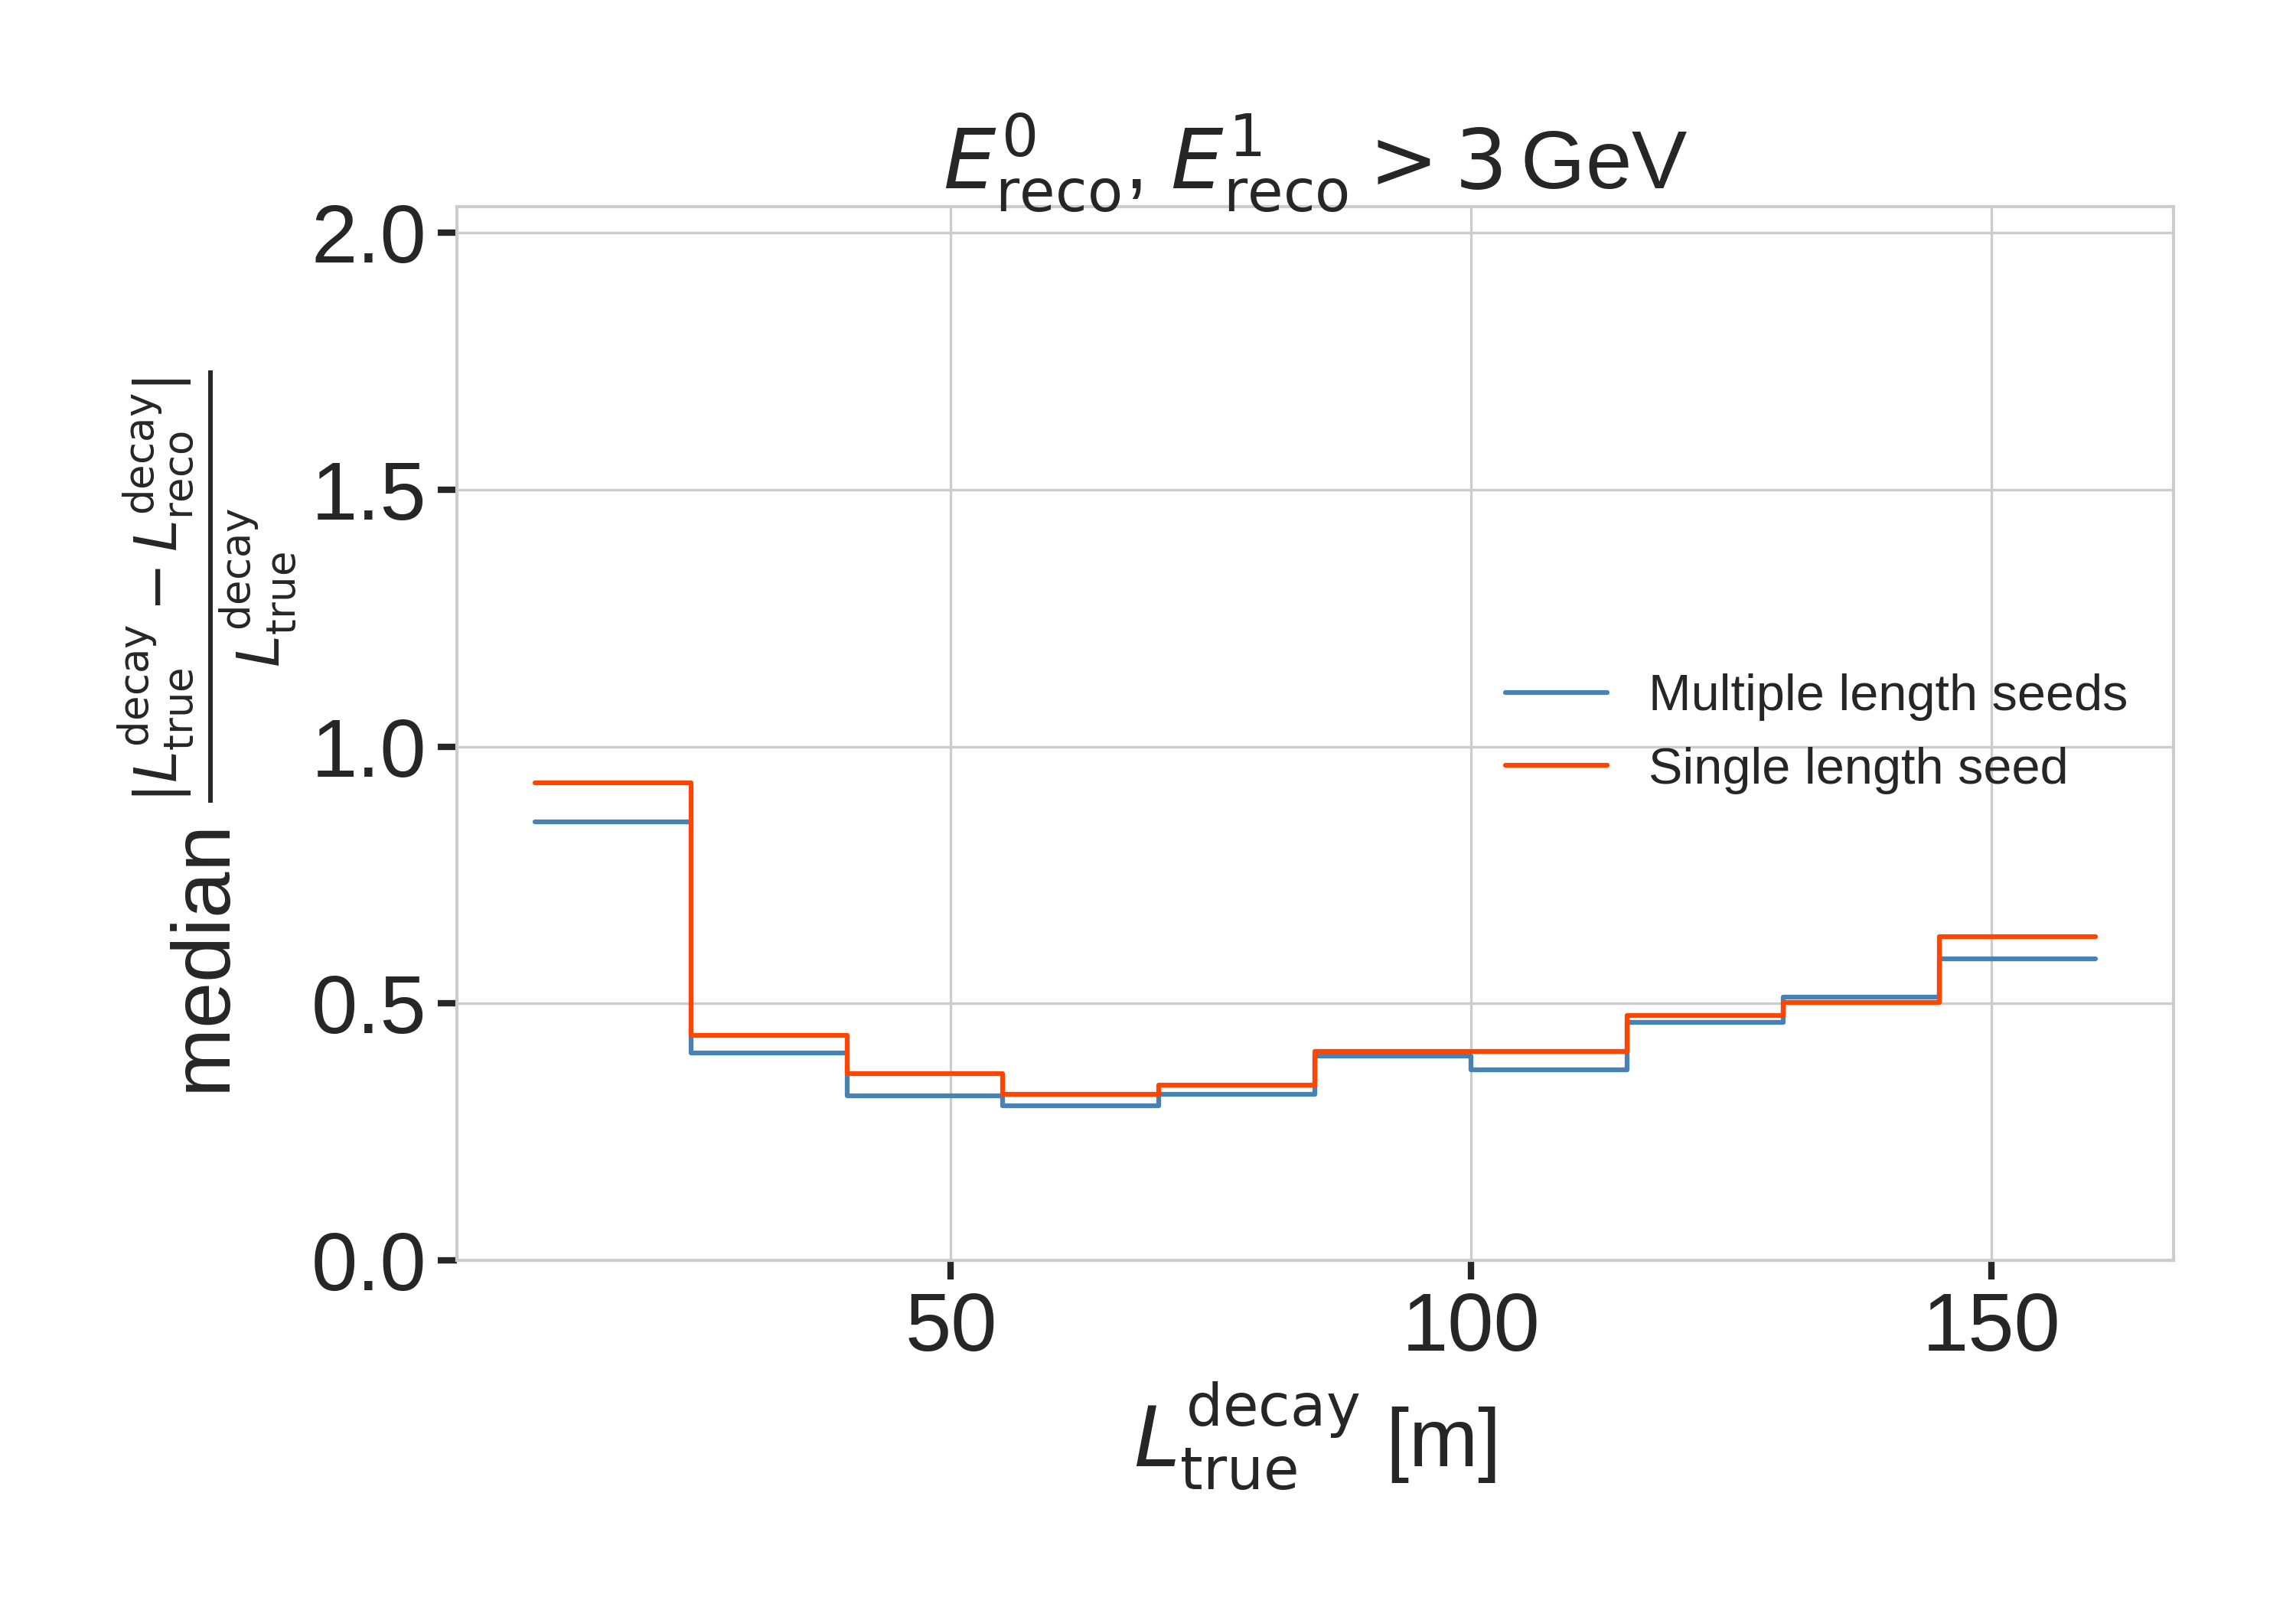
\includegraphics[width=0.49\linewidth]{figures/results/190605_reco_optimization/decay_length_seeding_median_decay_length_resolution_Good + L7 + reco E1,E2 above 3_fix_y.png}
    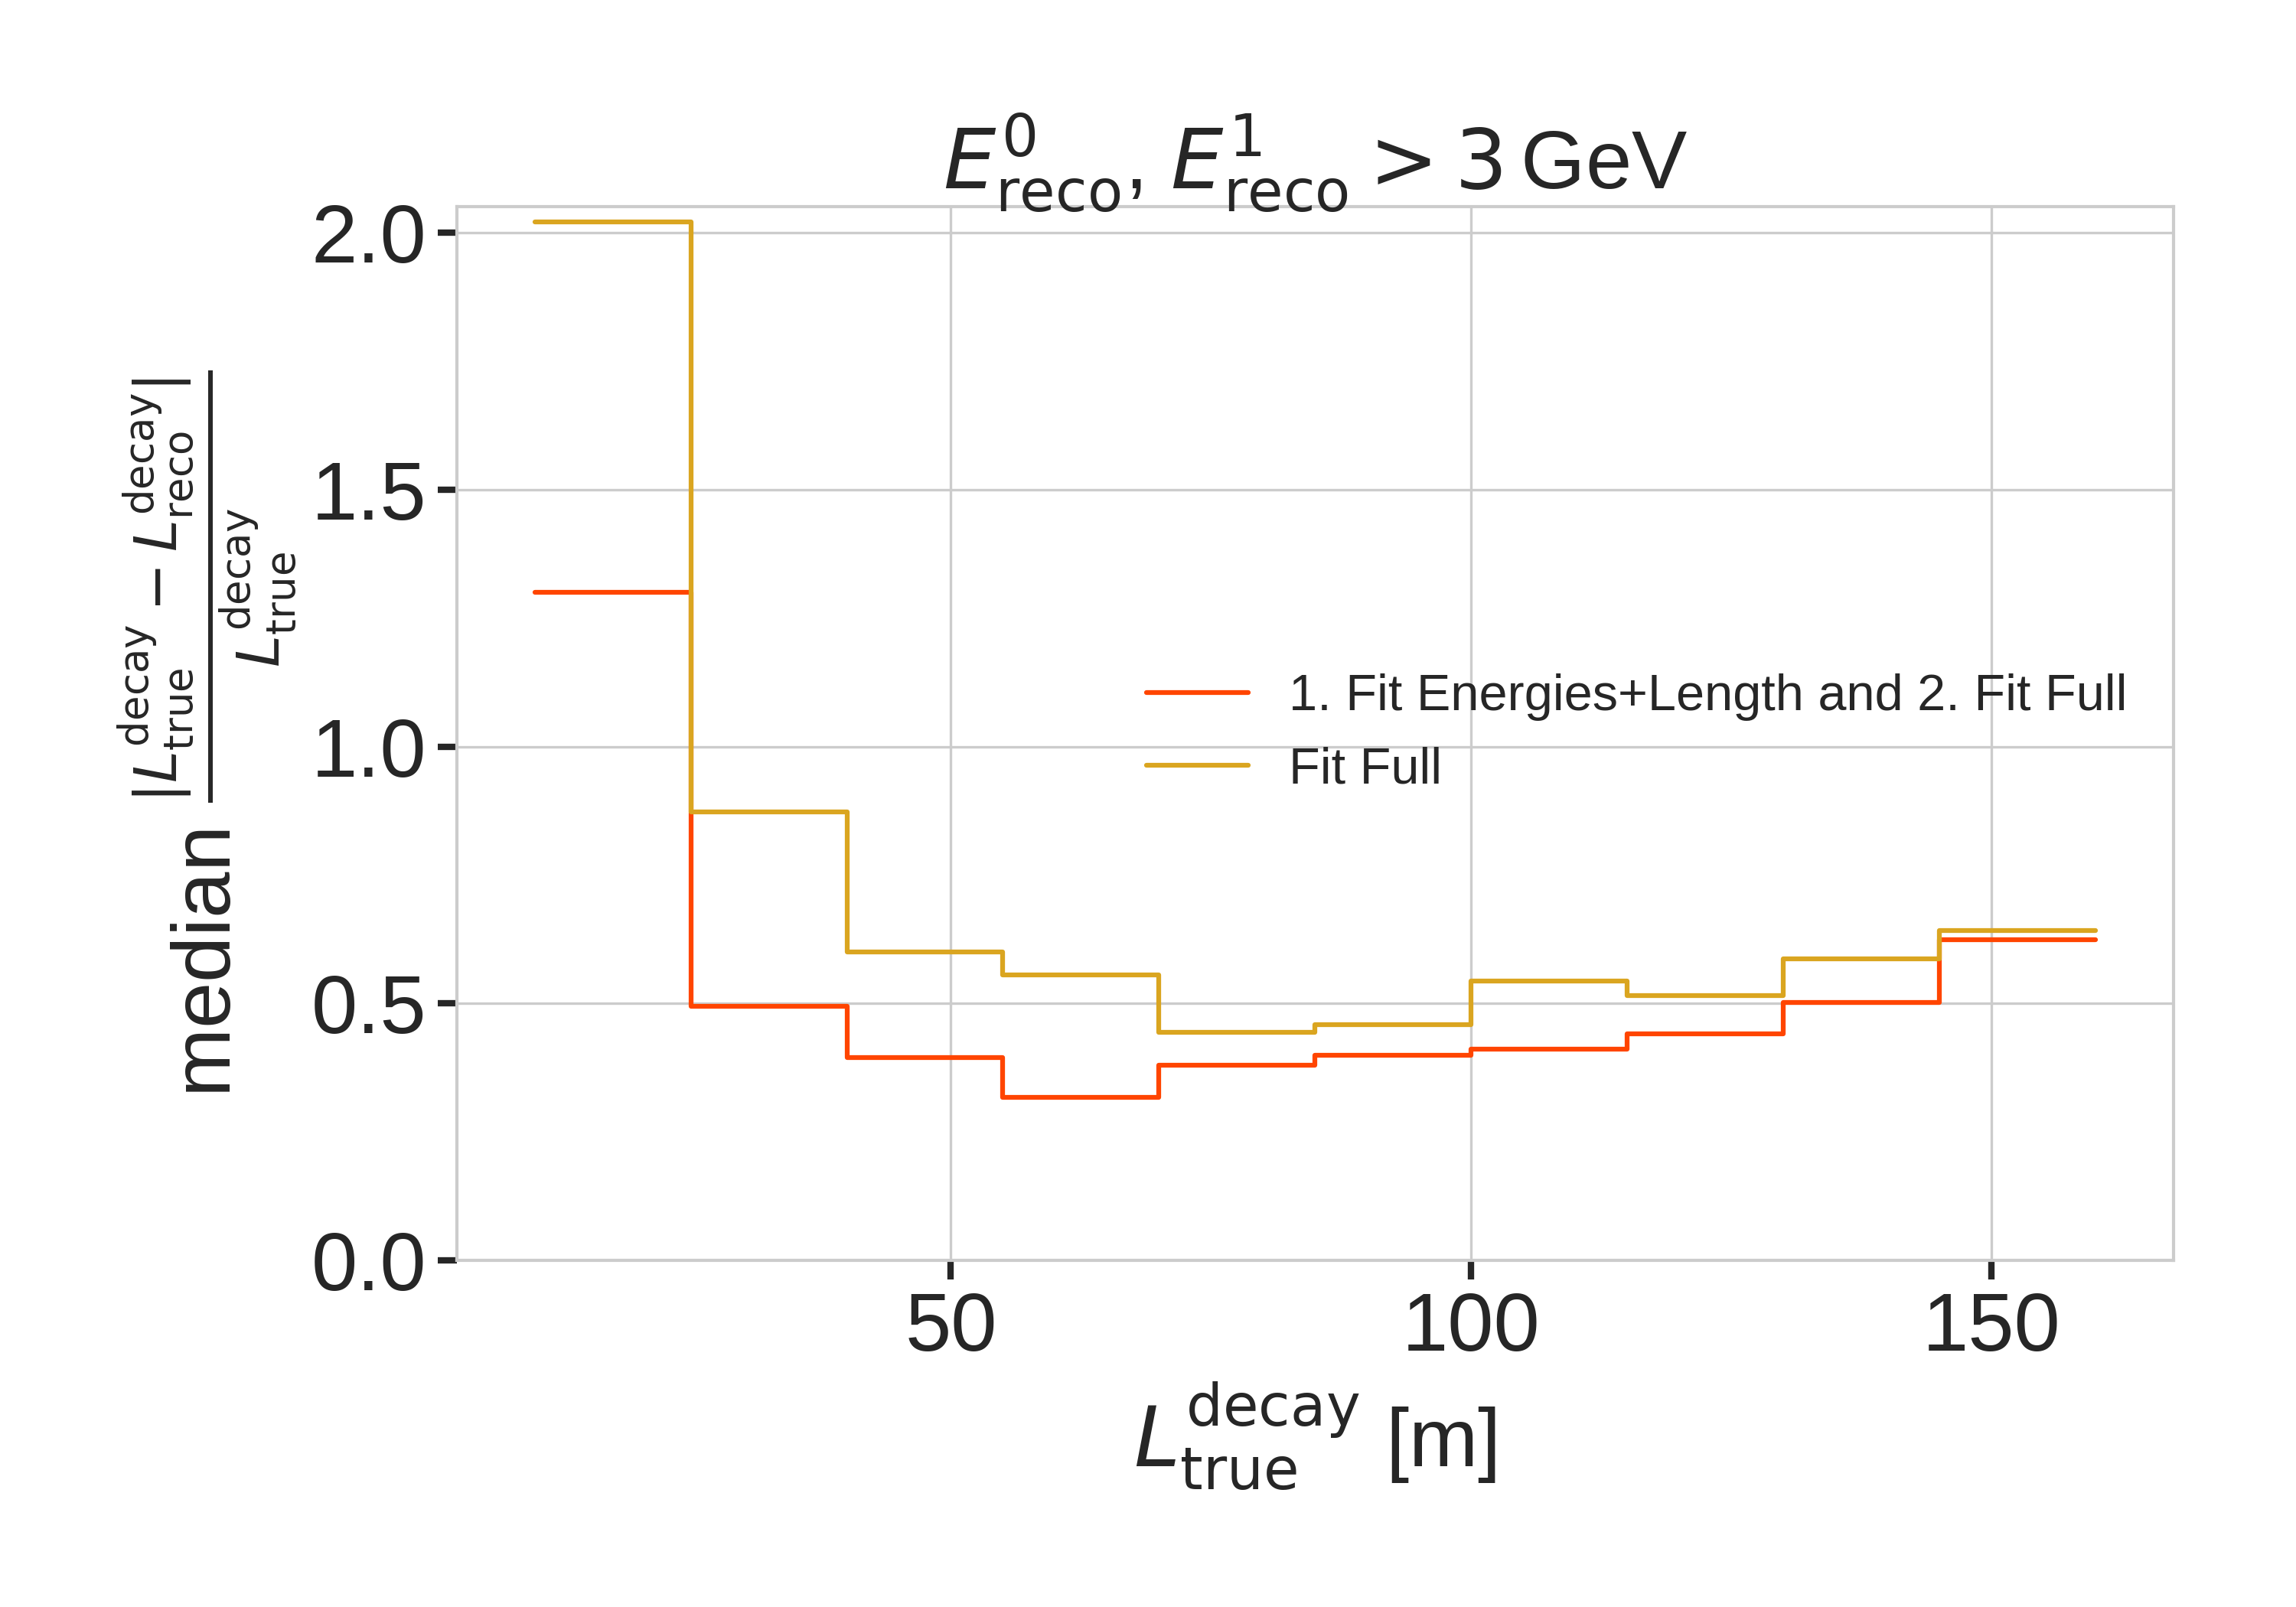
\includegraphics[width=0.49\linewidth]{figures/results/190605_reco_optimization/fit_routine_splitting_median_decay_length_resolution_Good + L7 + reco E1,E2 above 3_fix_y.png}
    \caption[]{}
    % \caption{Decay length resolution versus true decay length comparing the same fit routine seeded with just the seed decay length (Single length seed) and seeded with a decay length of 5\,m, 25\,m, 50\,m, 100\,m, and 200\,m (Multiple length seeds). This was done with older signal simulation set (190605) and the resolution is unweighted.}
    % \caption{Decay length resolution versus true decay length comparing a full 9 paramters fit to an iterative approach where first the energies and the decay lenght are fitted, while fixing the other 7 parameters and then the full fit is performed. This was done with older signal simulation set (190605) and the resolution is unweighted.}
    \labfig{fit_routine_optimization}
\end{figure*}
\todo{fix caption of this figure}


\subsubsection{Fit Routine}

Because the length seed showed to have such a large impact on the reconstruction performance, a more sophisticated fit routine, than just fitting all 9 parameters at once, was tested. In a first fit iteration, some parameters are fixed and the resulting best fit point is used to fit all 9 parameters in a second iteration. In the right part of \reffig{fit_routine_optimization} it can be seen how a fit split into two consecutive steps, where the first step fits only both cascade energies and the decay length and the second step fits the full 9 parameters, performs better as compared to a single, full 9 parameter fit. The initial seed for both routines is the same.


\subsubsection{Minimizer Settings}

To investigate the effect of the minimizer used to find the best fit parameters, the reconstruction was performed using three different minimizers, which were easily accessible within the reconstruction framework. The minimizers used were Minuit1 Simplex, Minuit2 Simplex, and Minuit2 Migrad. The results can be seen in \reffig{minimizer_optimization}, where the Minuit1 Simplex minimizer performs best. The initial idea was to test a global minimizer, or a routine that can find the rough position of the global minimum first and then a local minimizer to find the exact minimum, but unfortunately this was not possible with the minimizers available in the framework. From the three tested minimizers, Minuit1 Simplex performed best and was chosen as the default for the reconstruction. The comparision of the decay length resolutions can be seen in \reffig{minimizer_optimization}.


\begin{figure}
    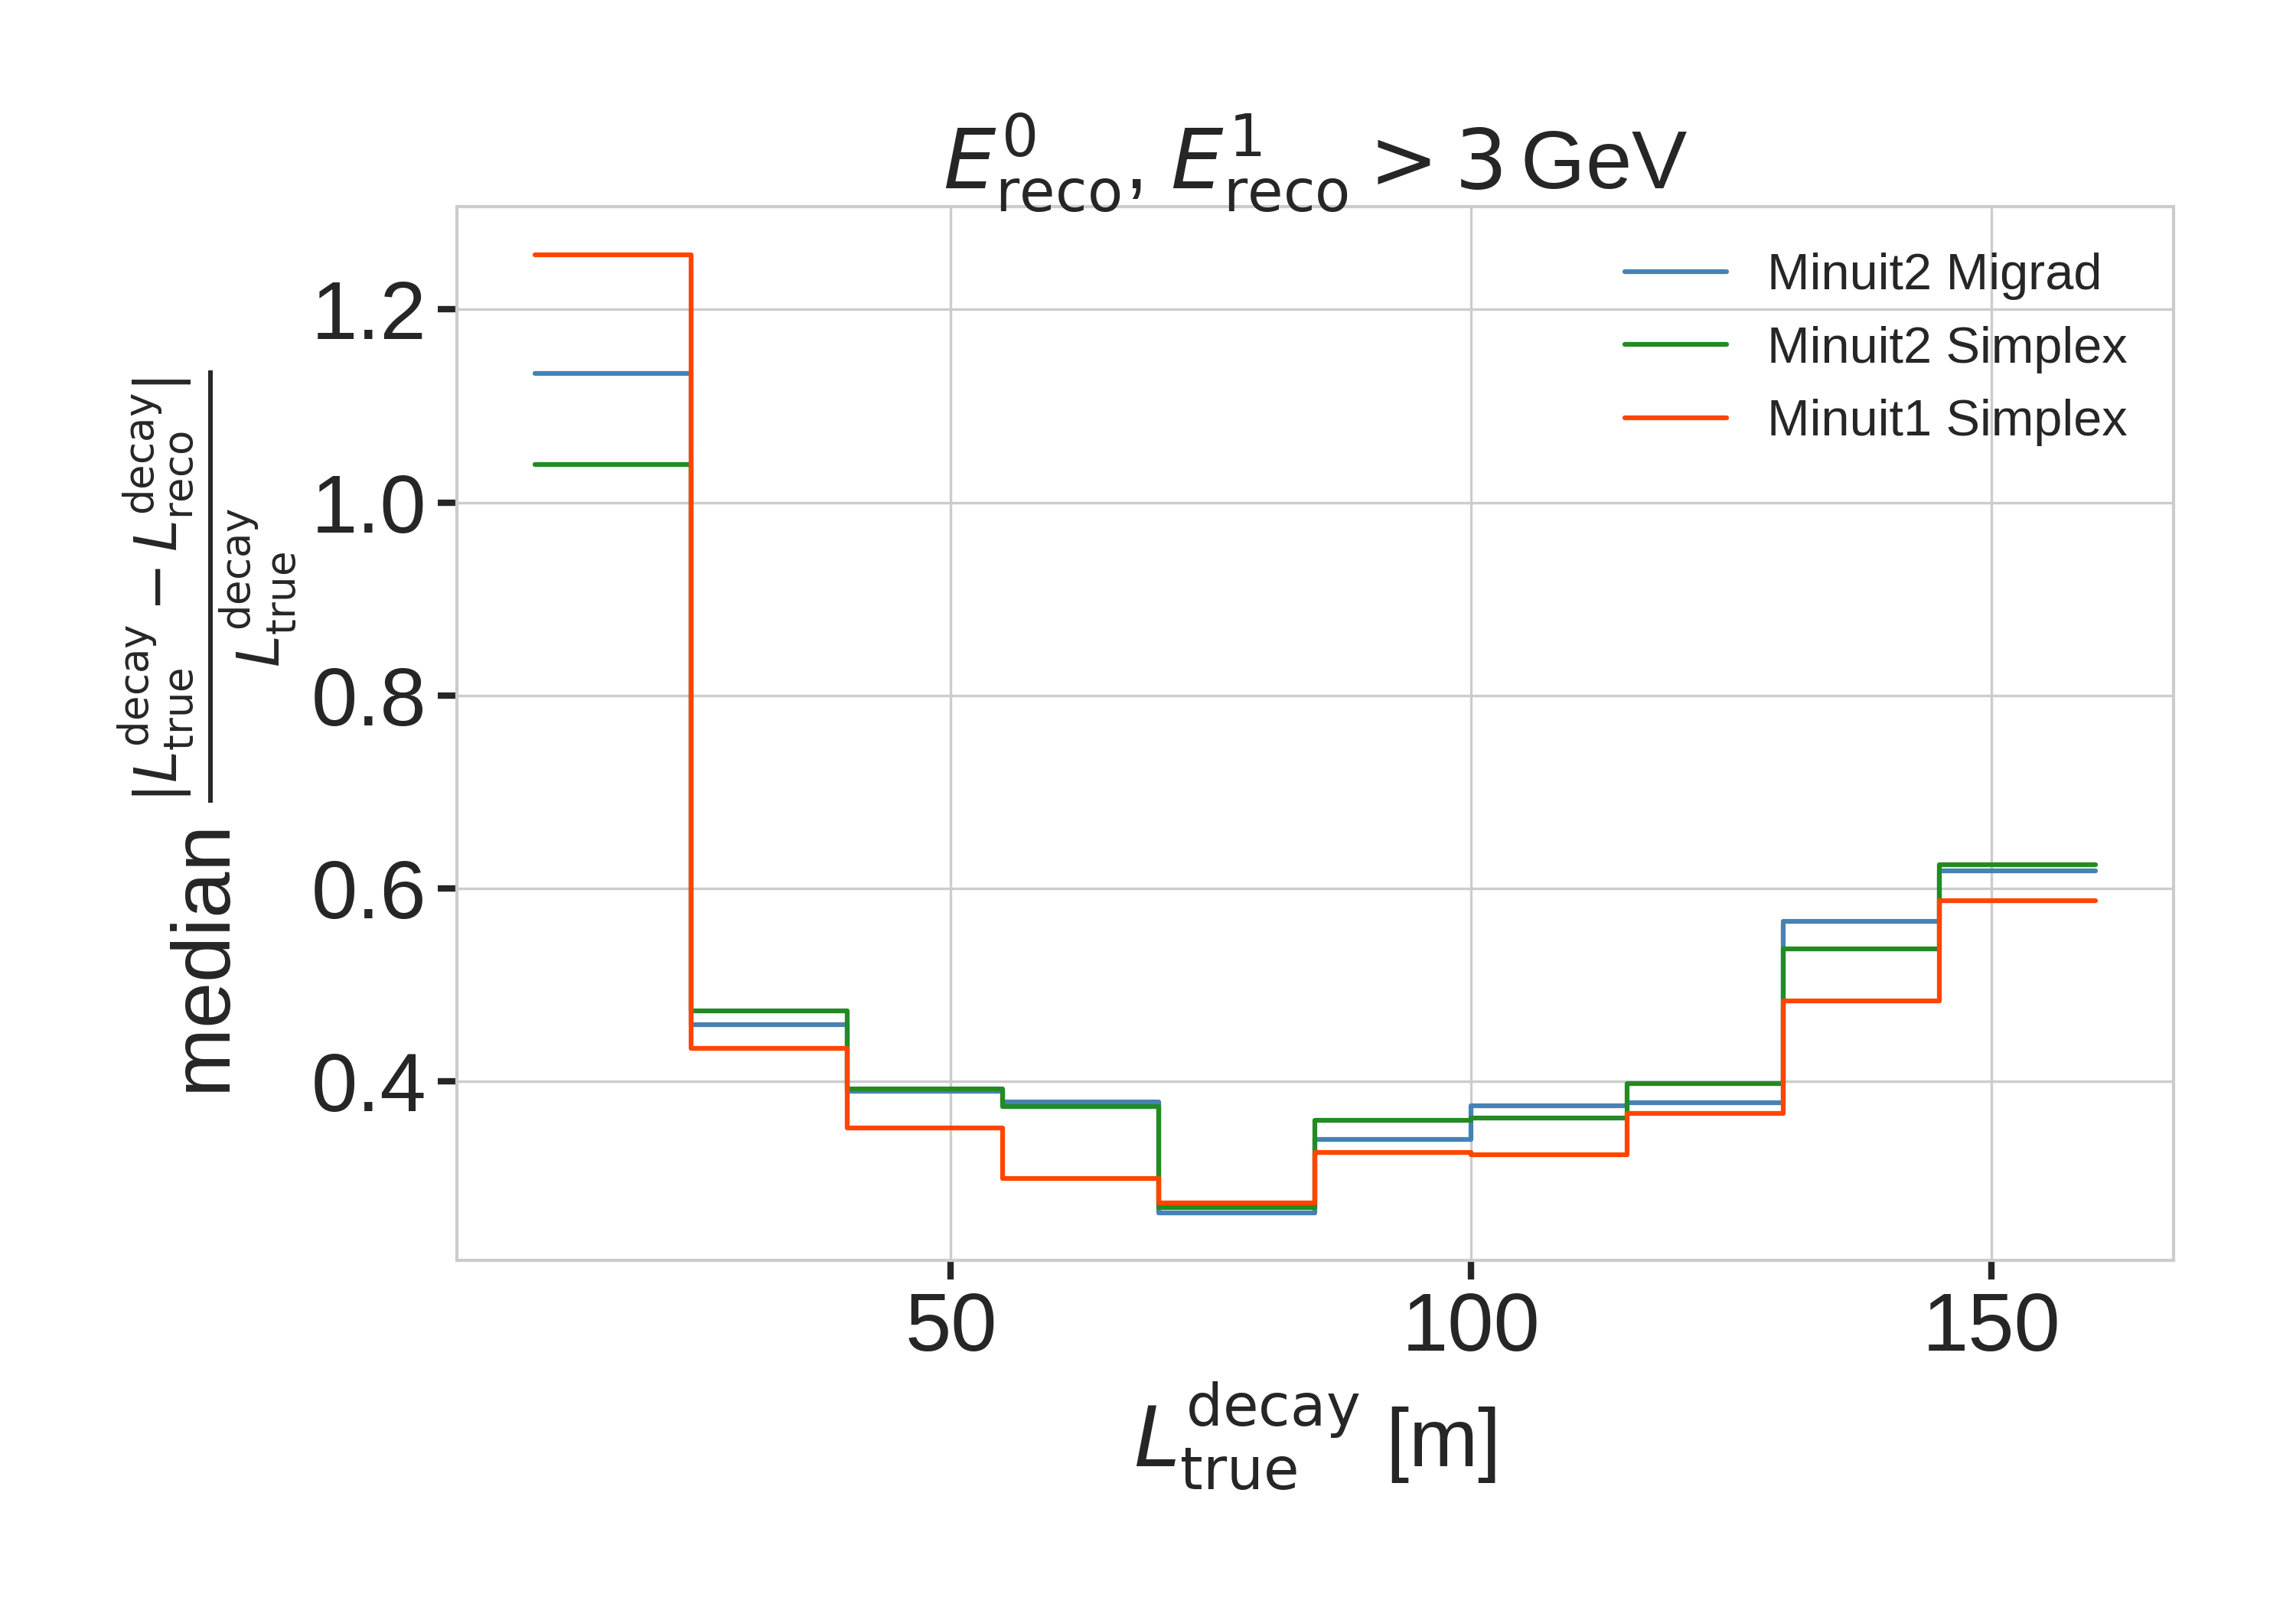
\includegraphics{figures/results/190605_reco_optimization/minimizer_checks_median_decay_length_resolution_Good + L7 + reco E1,E2 above 3.png}
    \caption[short]{title}
    % \caption{Decay length resolution versus true decay length comparing the same fit routine performed with a different minimizer. These are the minimizers accessible with the Millipede framework. The (obvious) settings were chosen to be the same, but there might still be some hidden differences explaining the discrepency between the Minuit1 and Minuit2 implementation of Simplex. This was done with older signal simulation set (190605) and the resolution is unweighted.}
    \labfig{minimizer_optimization}
\end{figure}

\todo{fix caption of this figure}


\subsubsection{Reconstruction Chain}

The chosen reconstruction chain used to test the performance of the detector to observe low energetic double cascades is the following; Minuit1 Simplex is used as the minimizer, the decay length is seeded with 3 different values, 0.5x, 1.0x, and 1.5x the length of the track reconstruction, and the fit routine is split into two steps, where the first step fits the energies and the decay length and the second step fits the full 9 parameters. In the first step, the number of time bins in \refeq{millipede_likelihood} is set to 1, so just the number of photons and their spatial information is used. The second step is seeded with the best results from the first fit and here the number of time bins is chosen such that each photon falls into a separate time bin, which means all time information is used. The average runtime per event is $\sim$\SI{16}{\second} on a single CPU core, but is very dependent on the number of photons observed in the event, since the likelihood calculation in the second step scales with this number and a table lookup has to be performed for each photon.\todo{Describe the results plots here for the first time, so I can come back to the observed features later? Or maybe drop them and just show them later?}


\begin{figure*}[h]
	\centering
    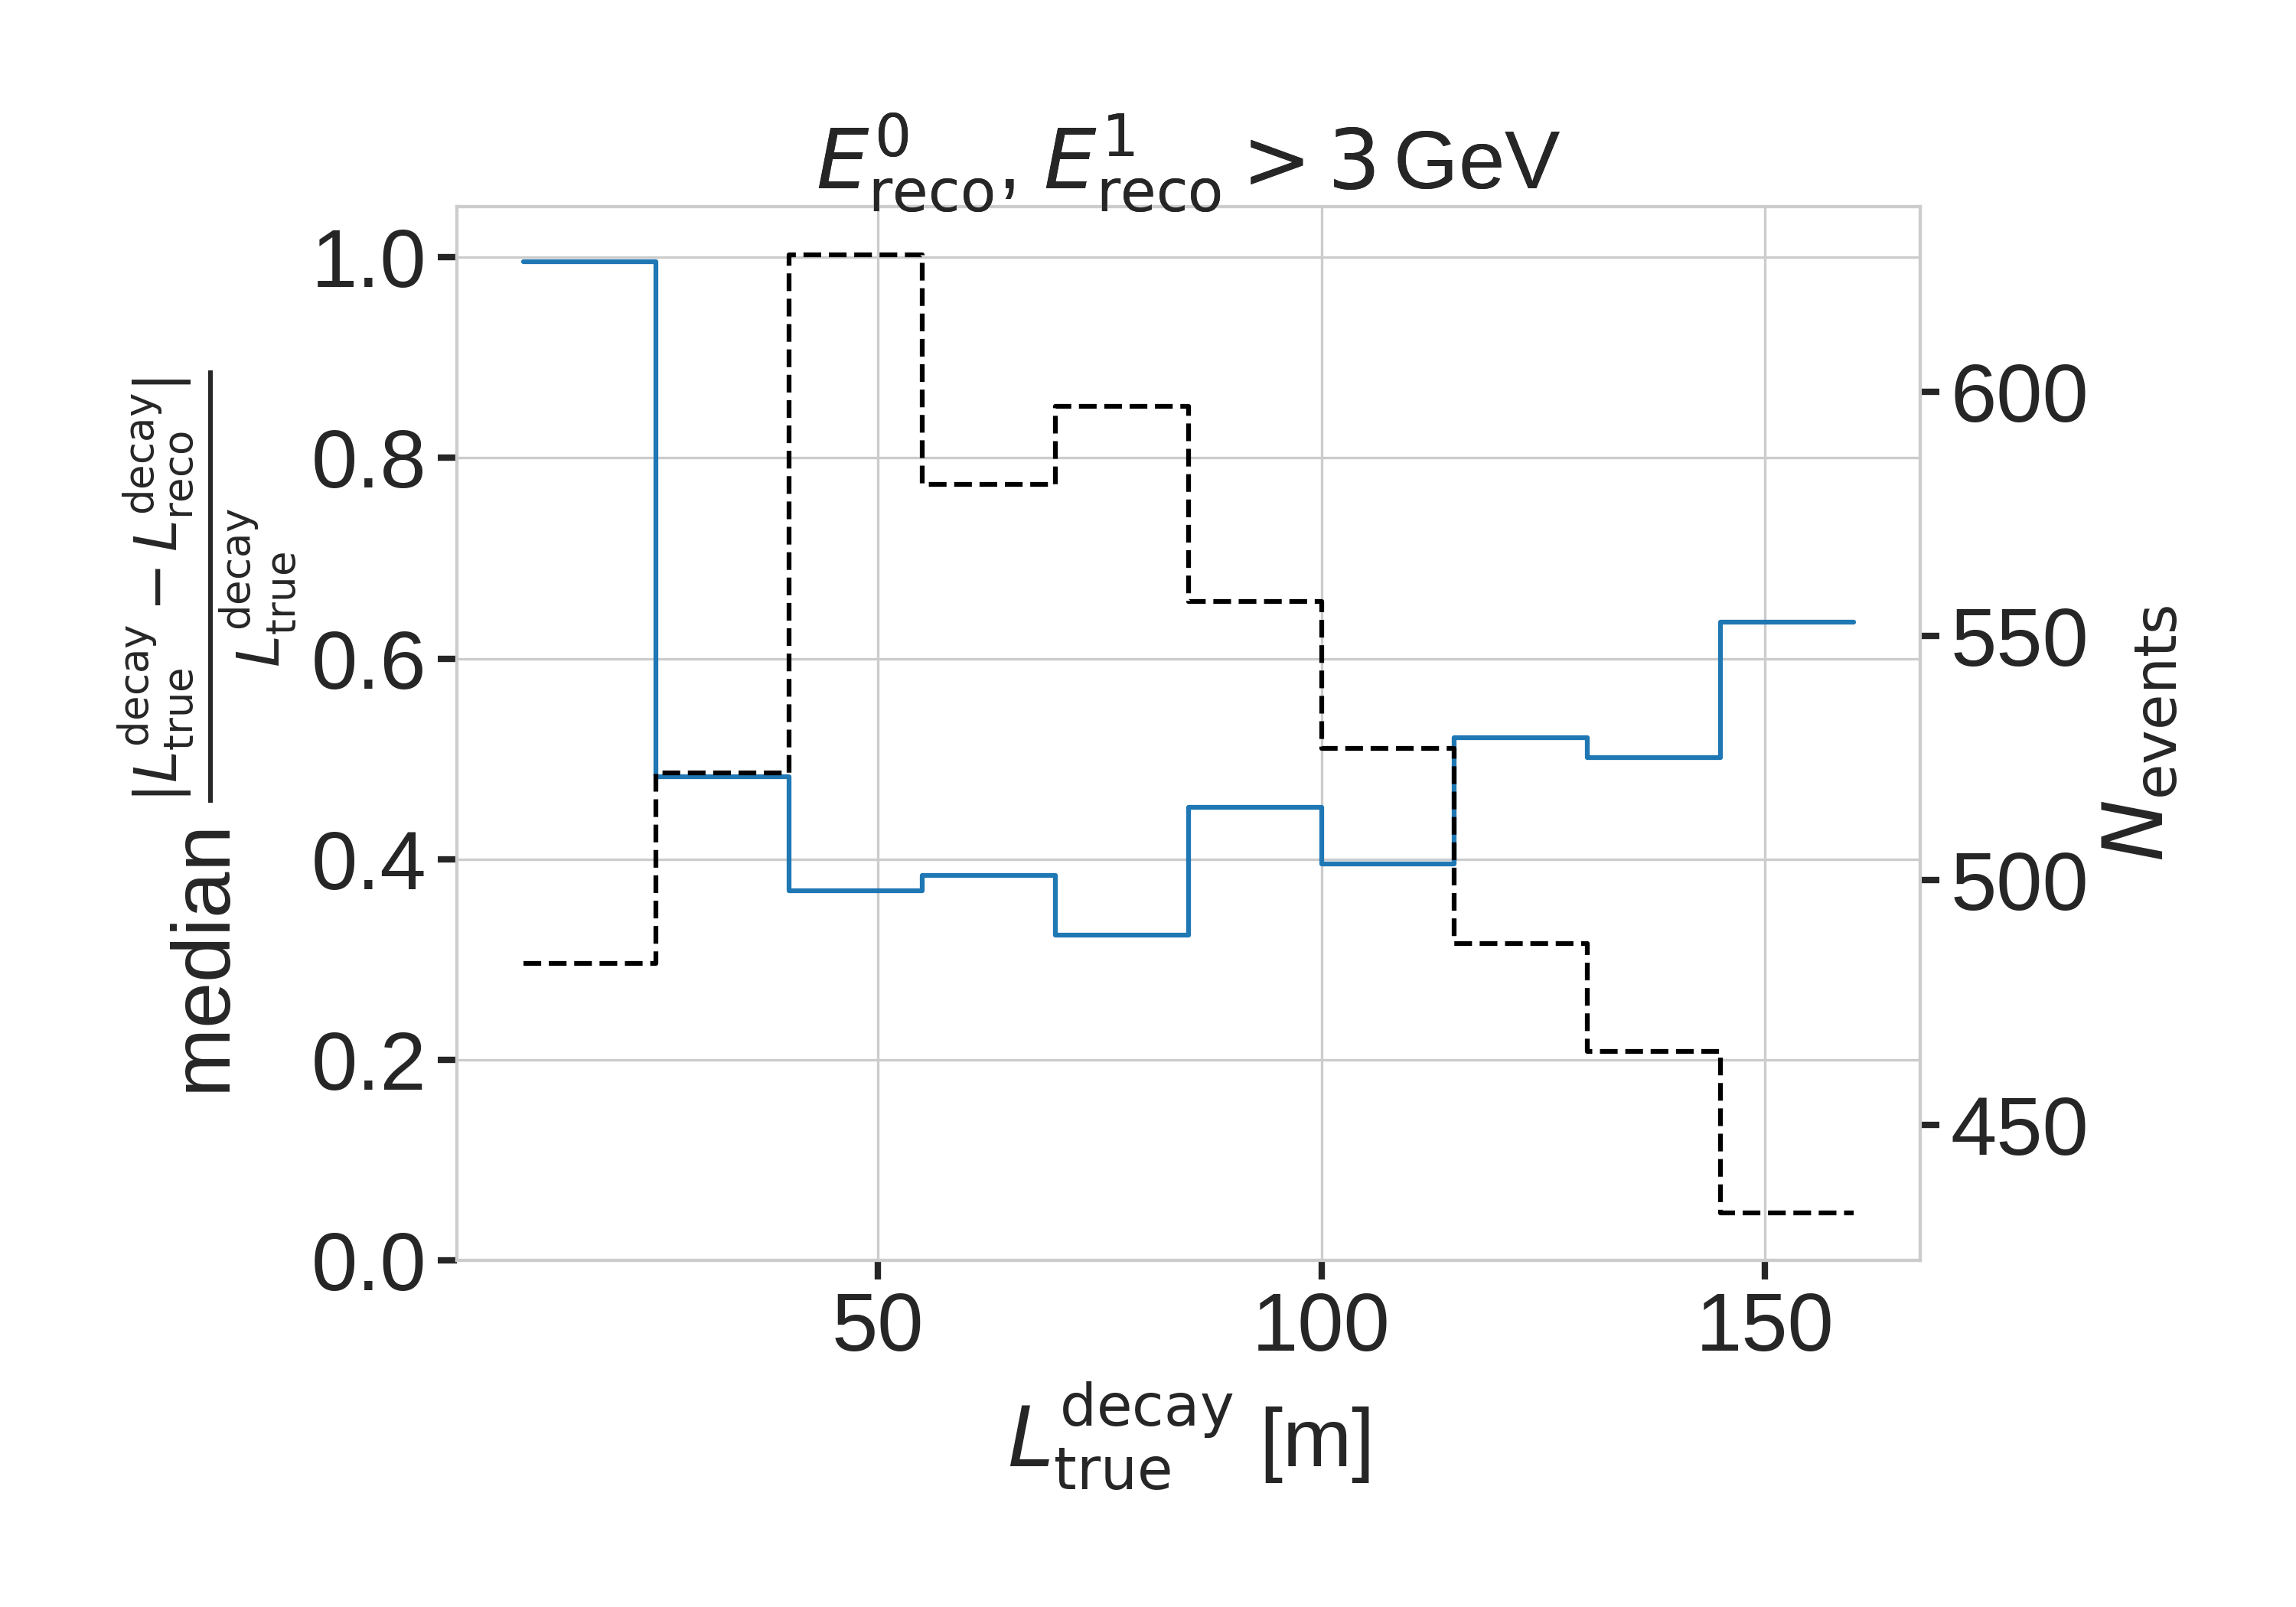
\includegraphics[width=0.49\linewidth]{figures/results/190605_reco_optimization/performance/selected_reco_chain_median_decay_length_resolution_Good + L7 + reco E1,E2 above 3_fix_y_n_events.png}
    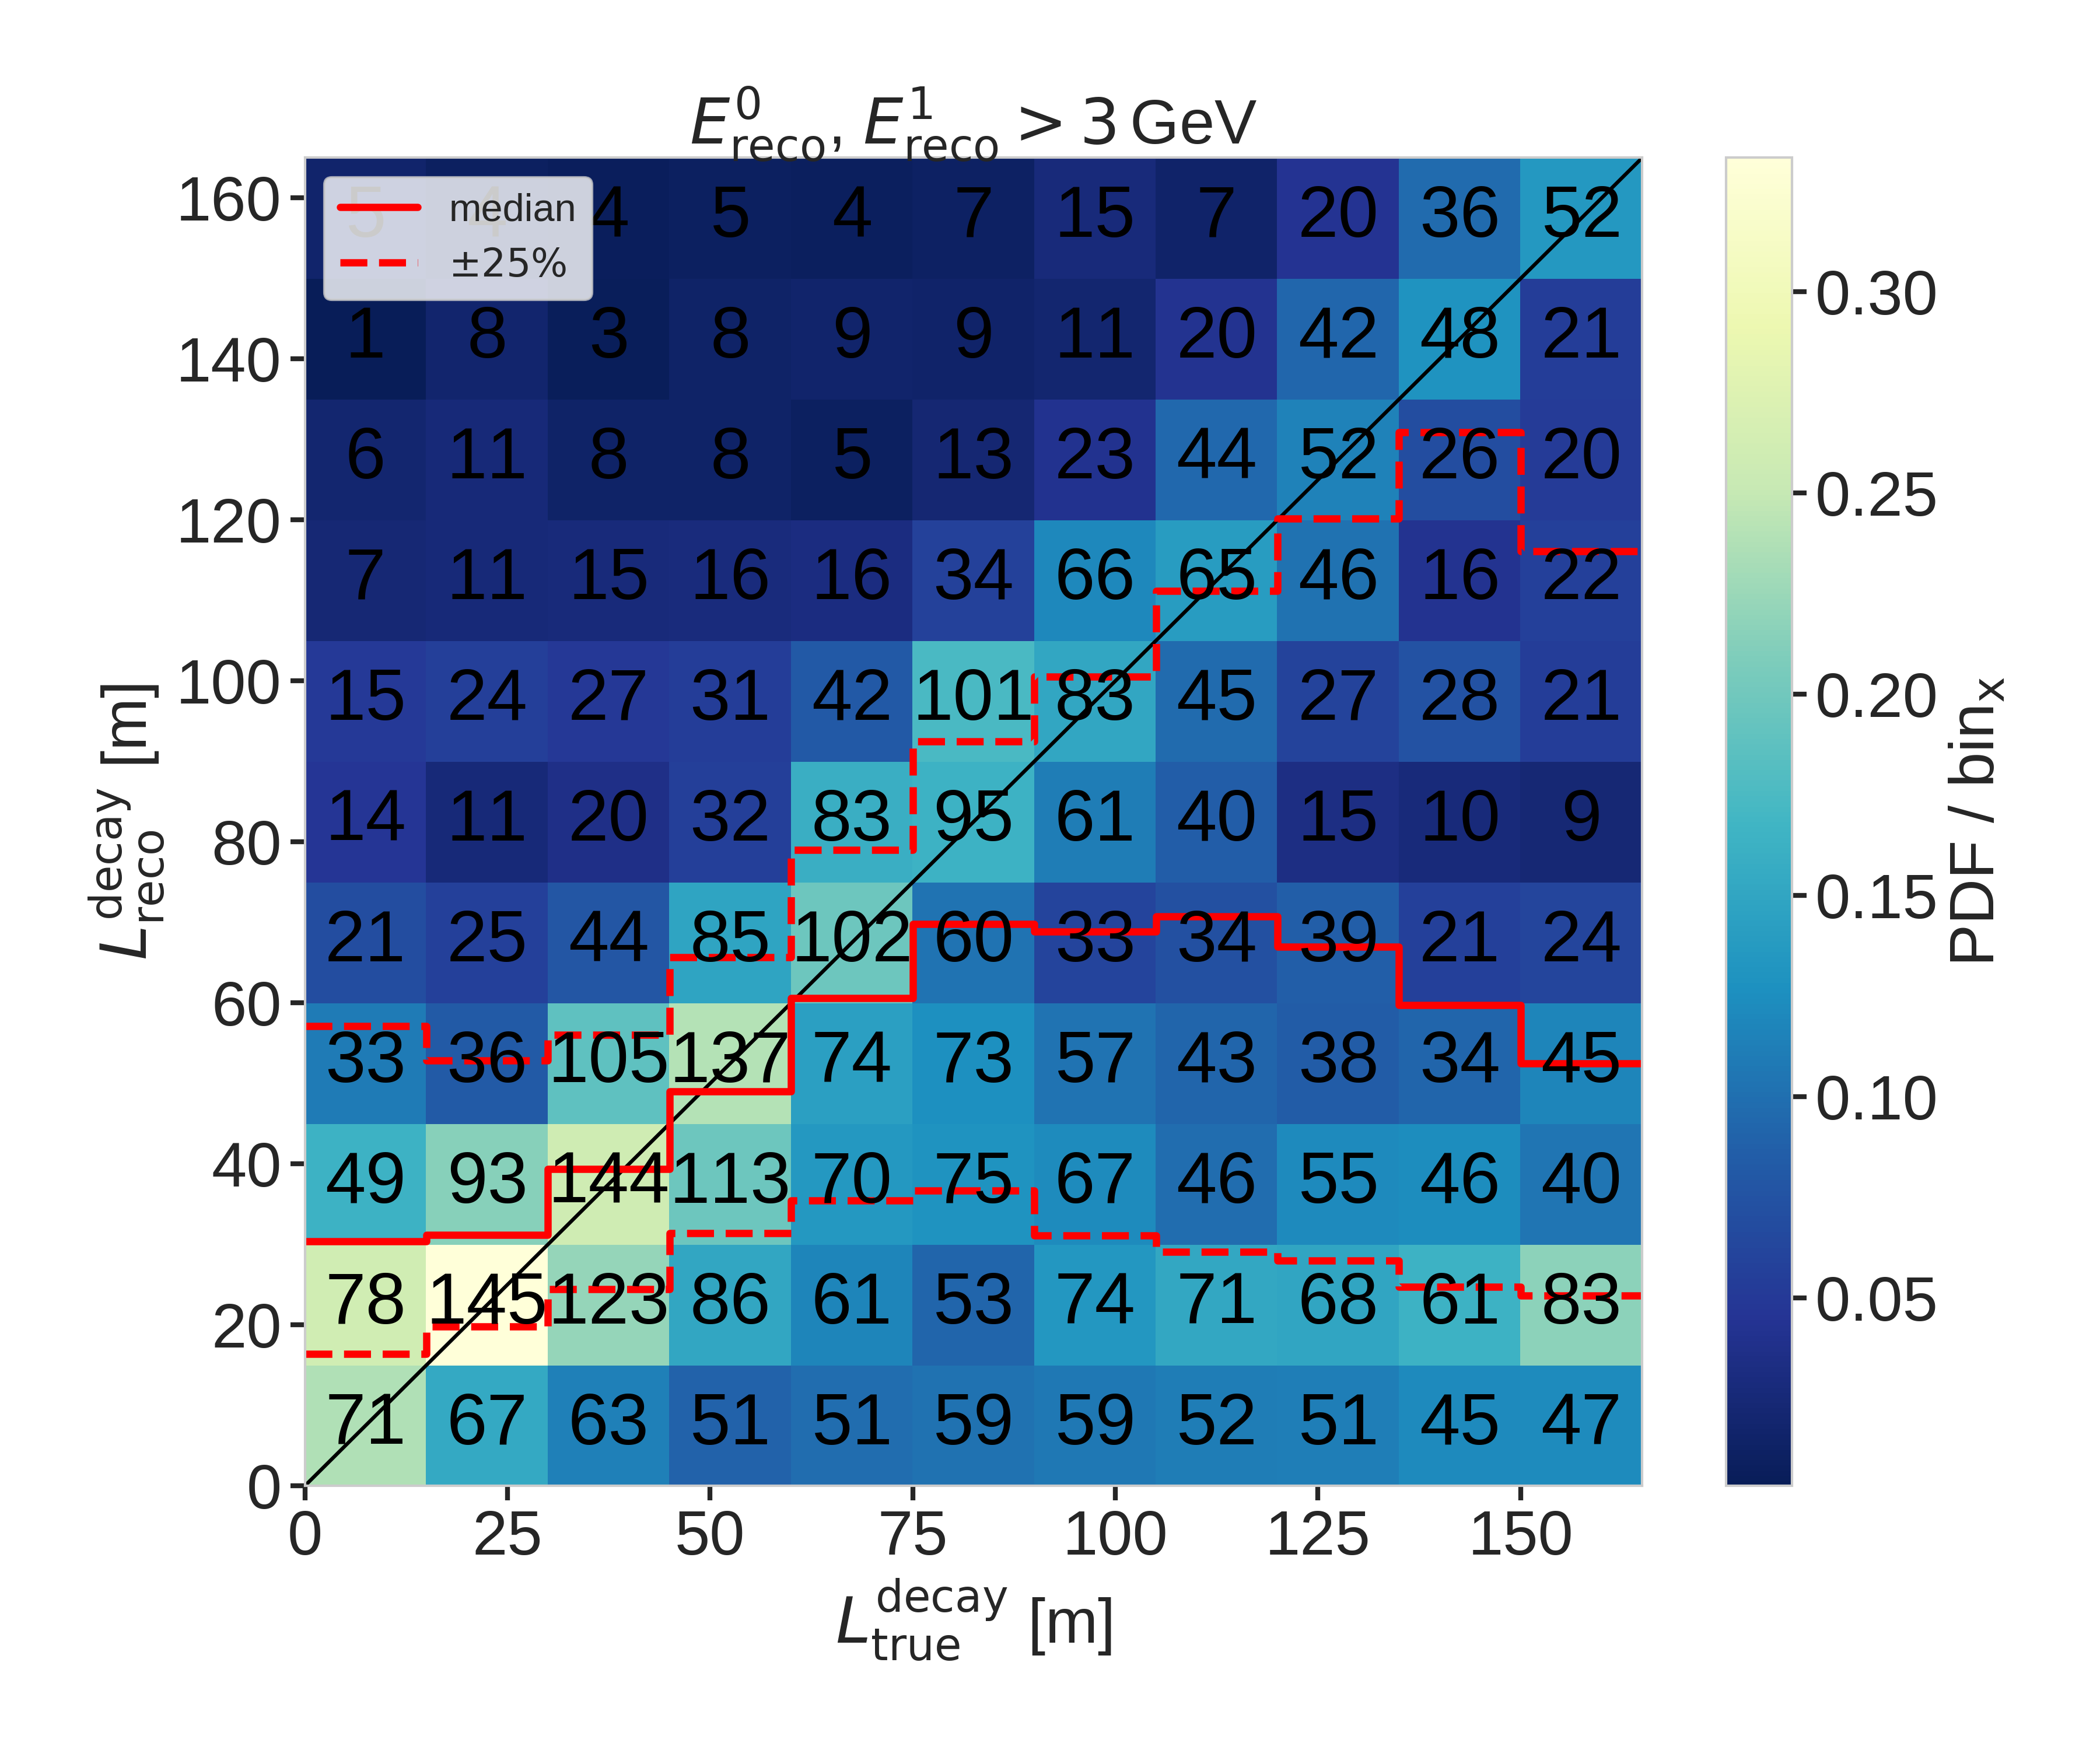
\includegraphics[width=0.49\linewidth]{figures/results/190605_reco_optimization/performance/selected_reco_chain_taupede_reco_decayL_vs_true_decayL_Good + L7 + reco E1,E2 above 3_step_contours.png}
    \caption[]{}
    \labfig{selected_routine_length_results}
\end{figure*}
\todo{fix caption of this figure}

\begin{figure*}[h]
	\centering
    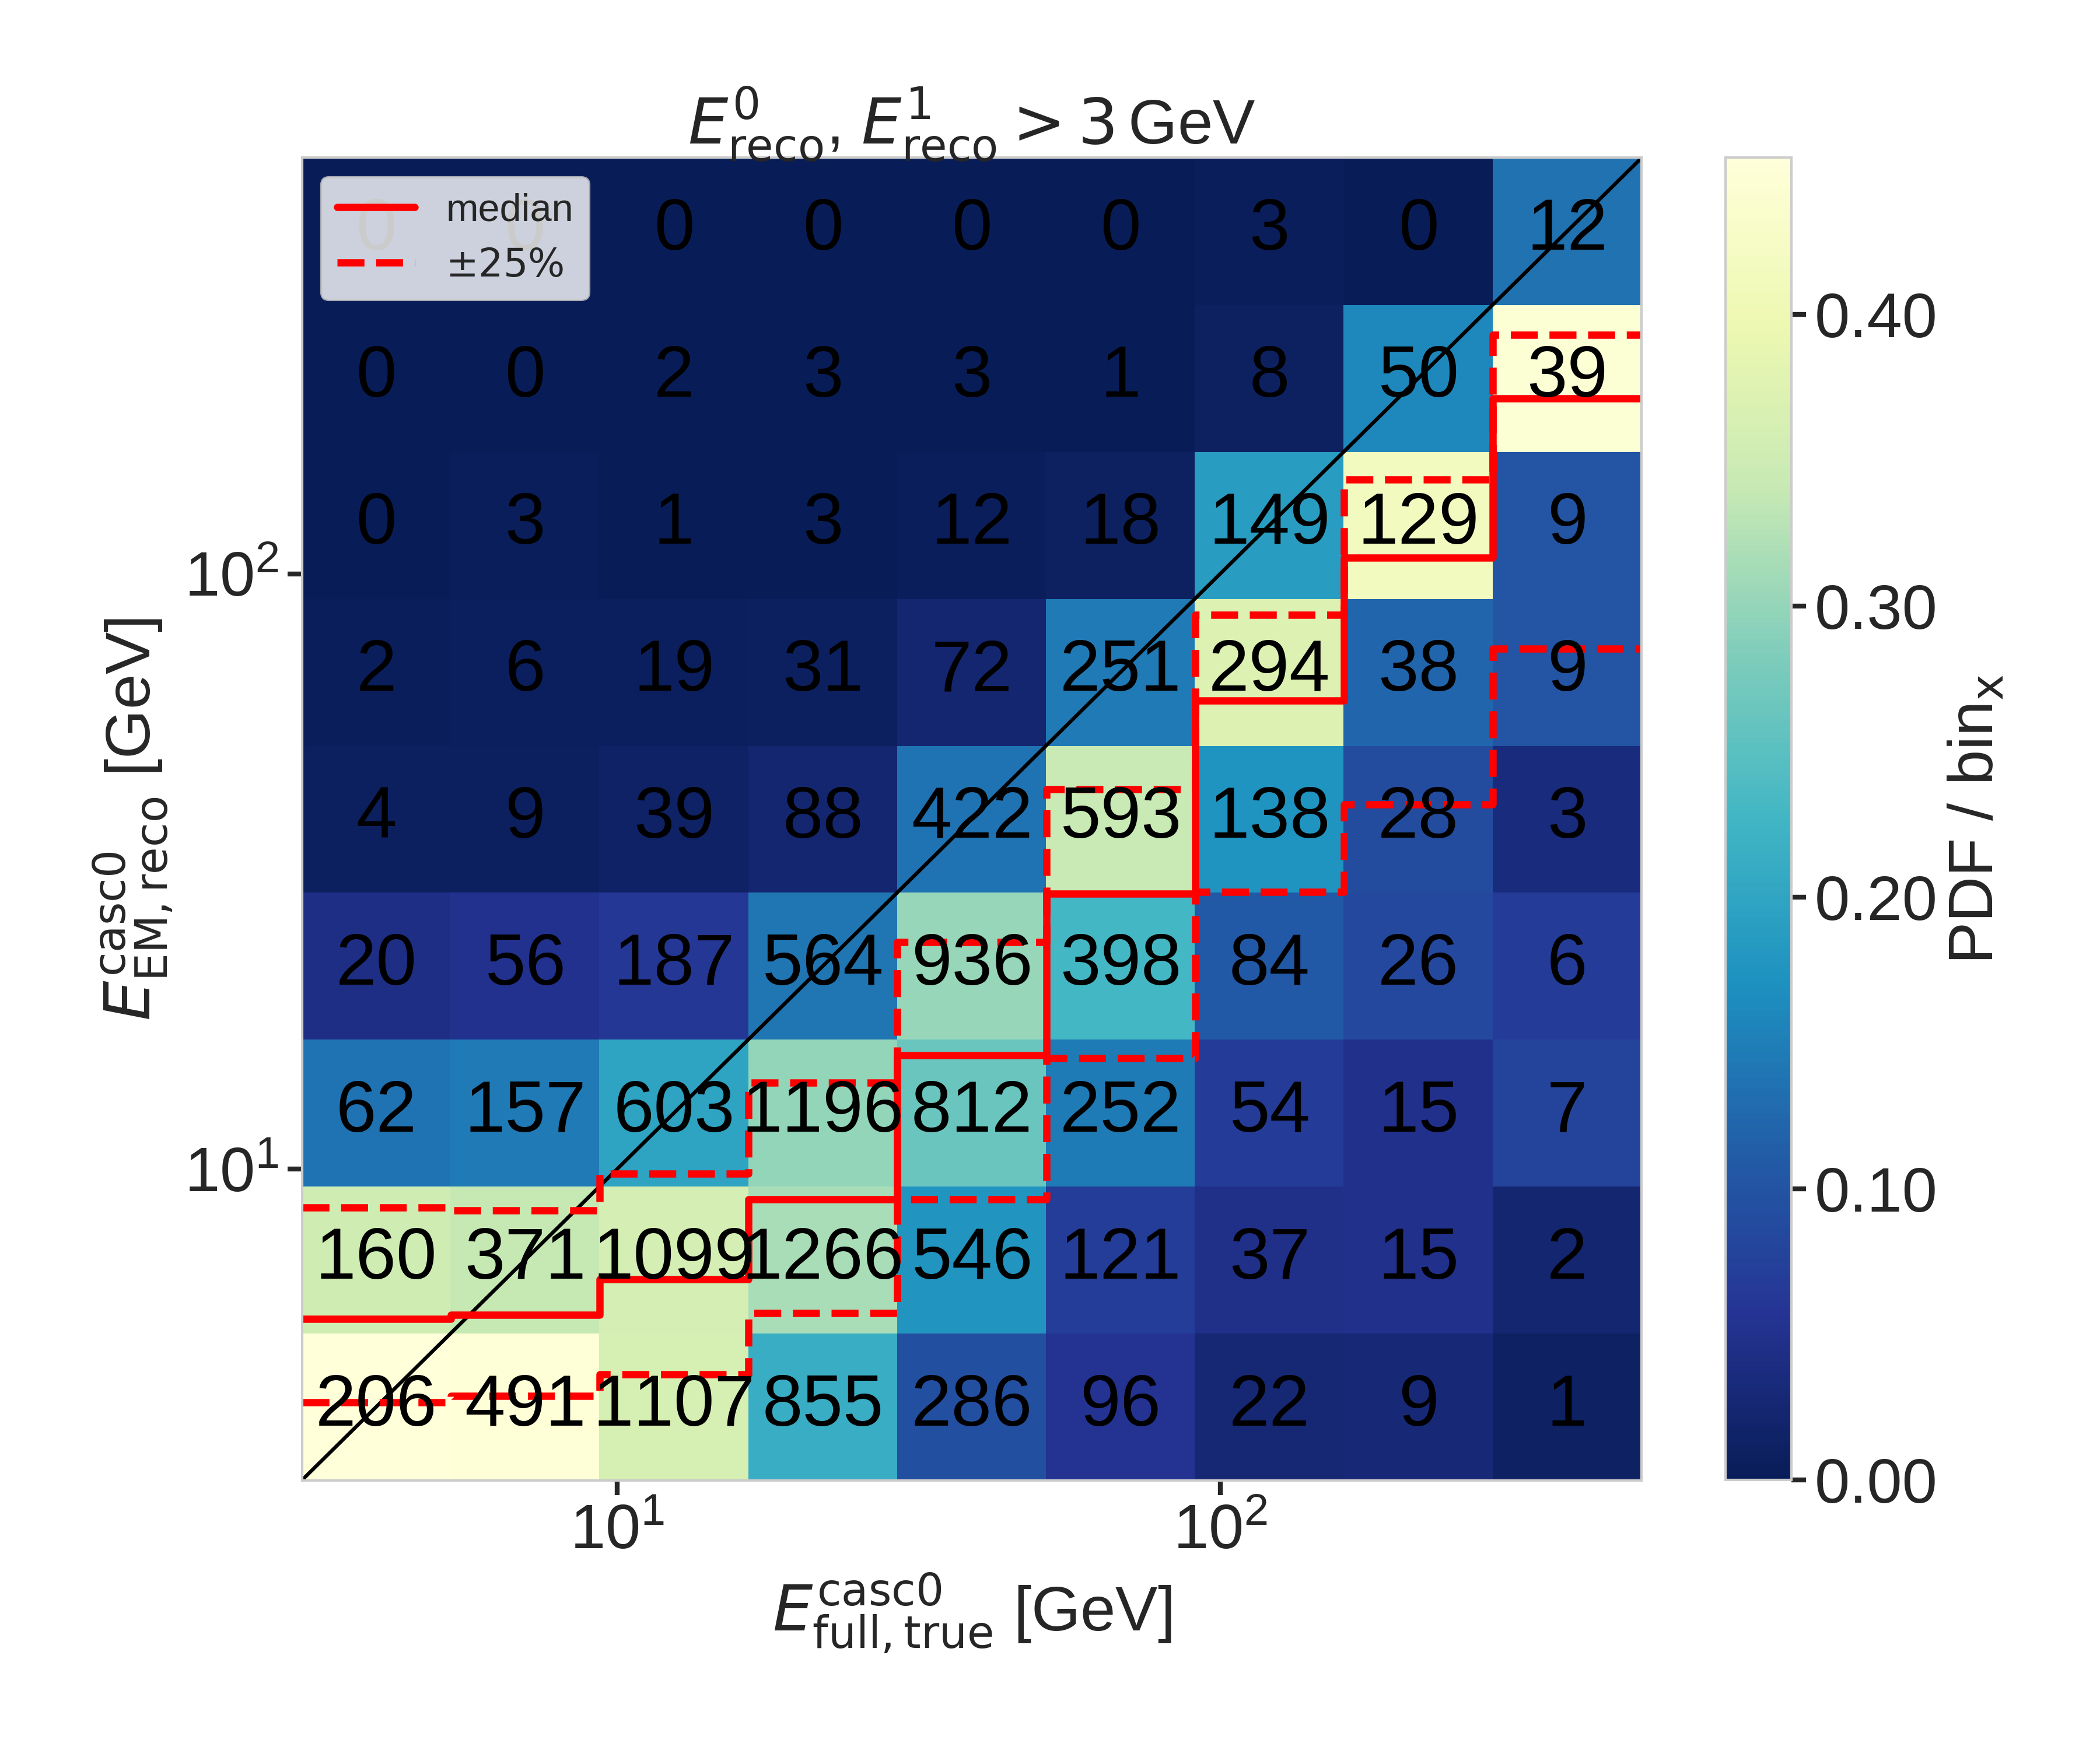
\includegraphics[width=0.49\linewidth]{figures/results/190605_reco_optimization/performance/selected_reco_chain_taupede_casc0_reco_energy_vs_casc0_true_energy_Good + L7 + reco E1,E2 above 3_step_contours.png}
    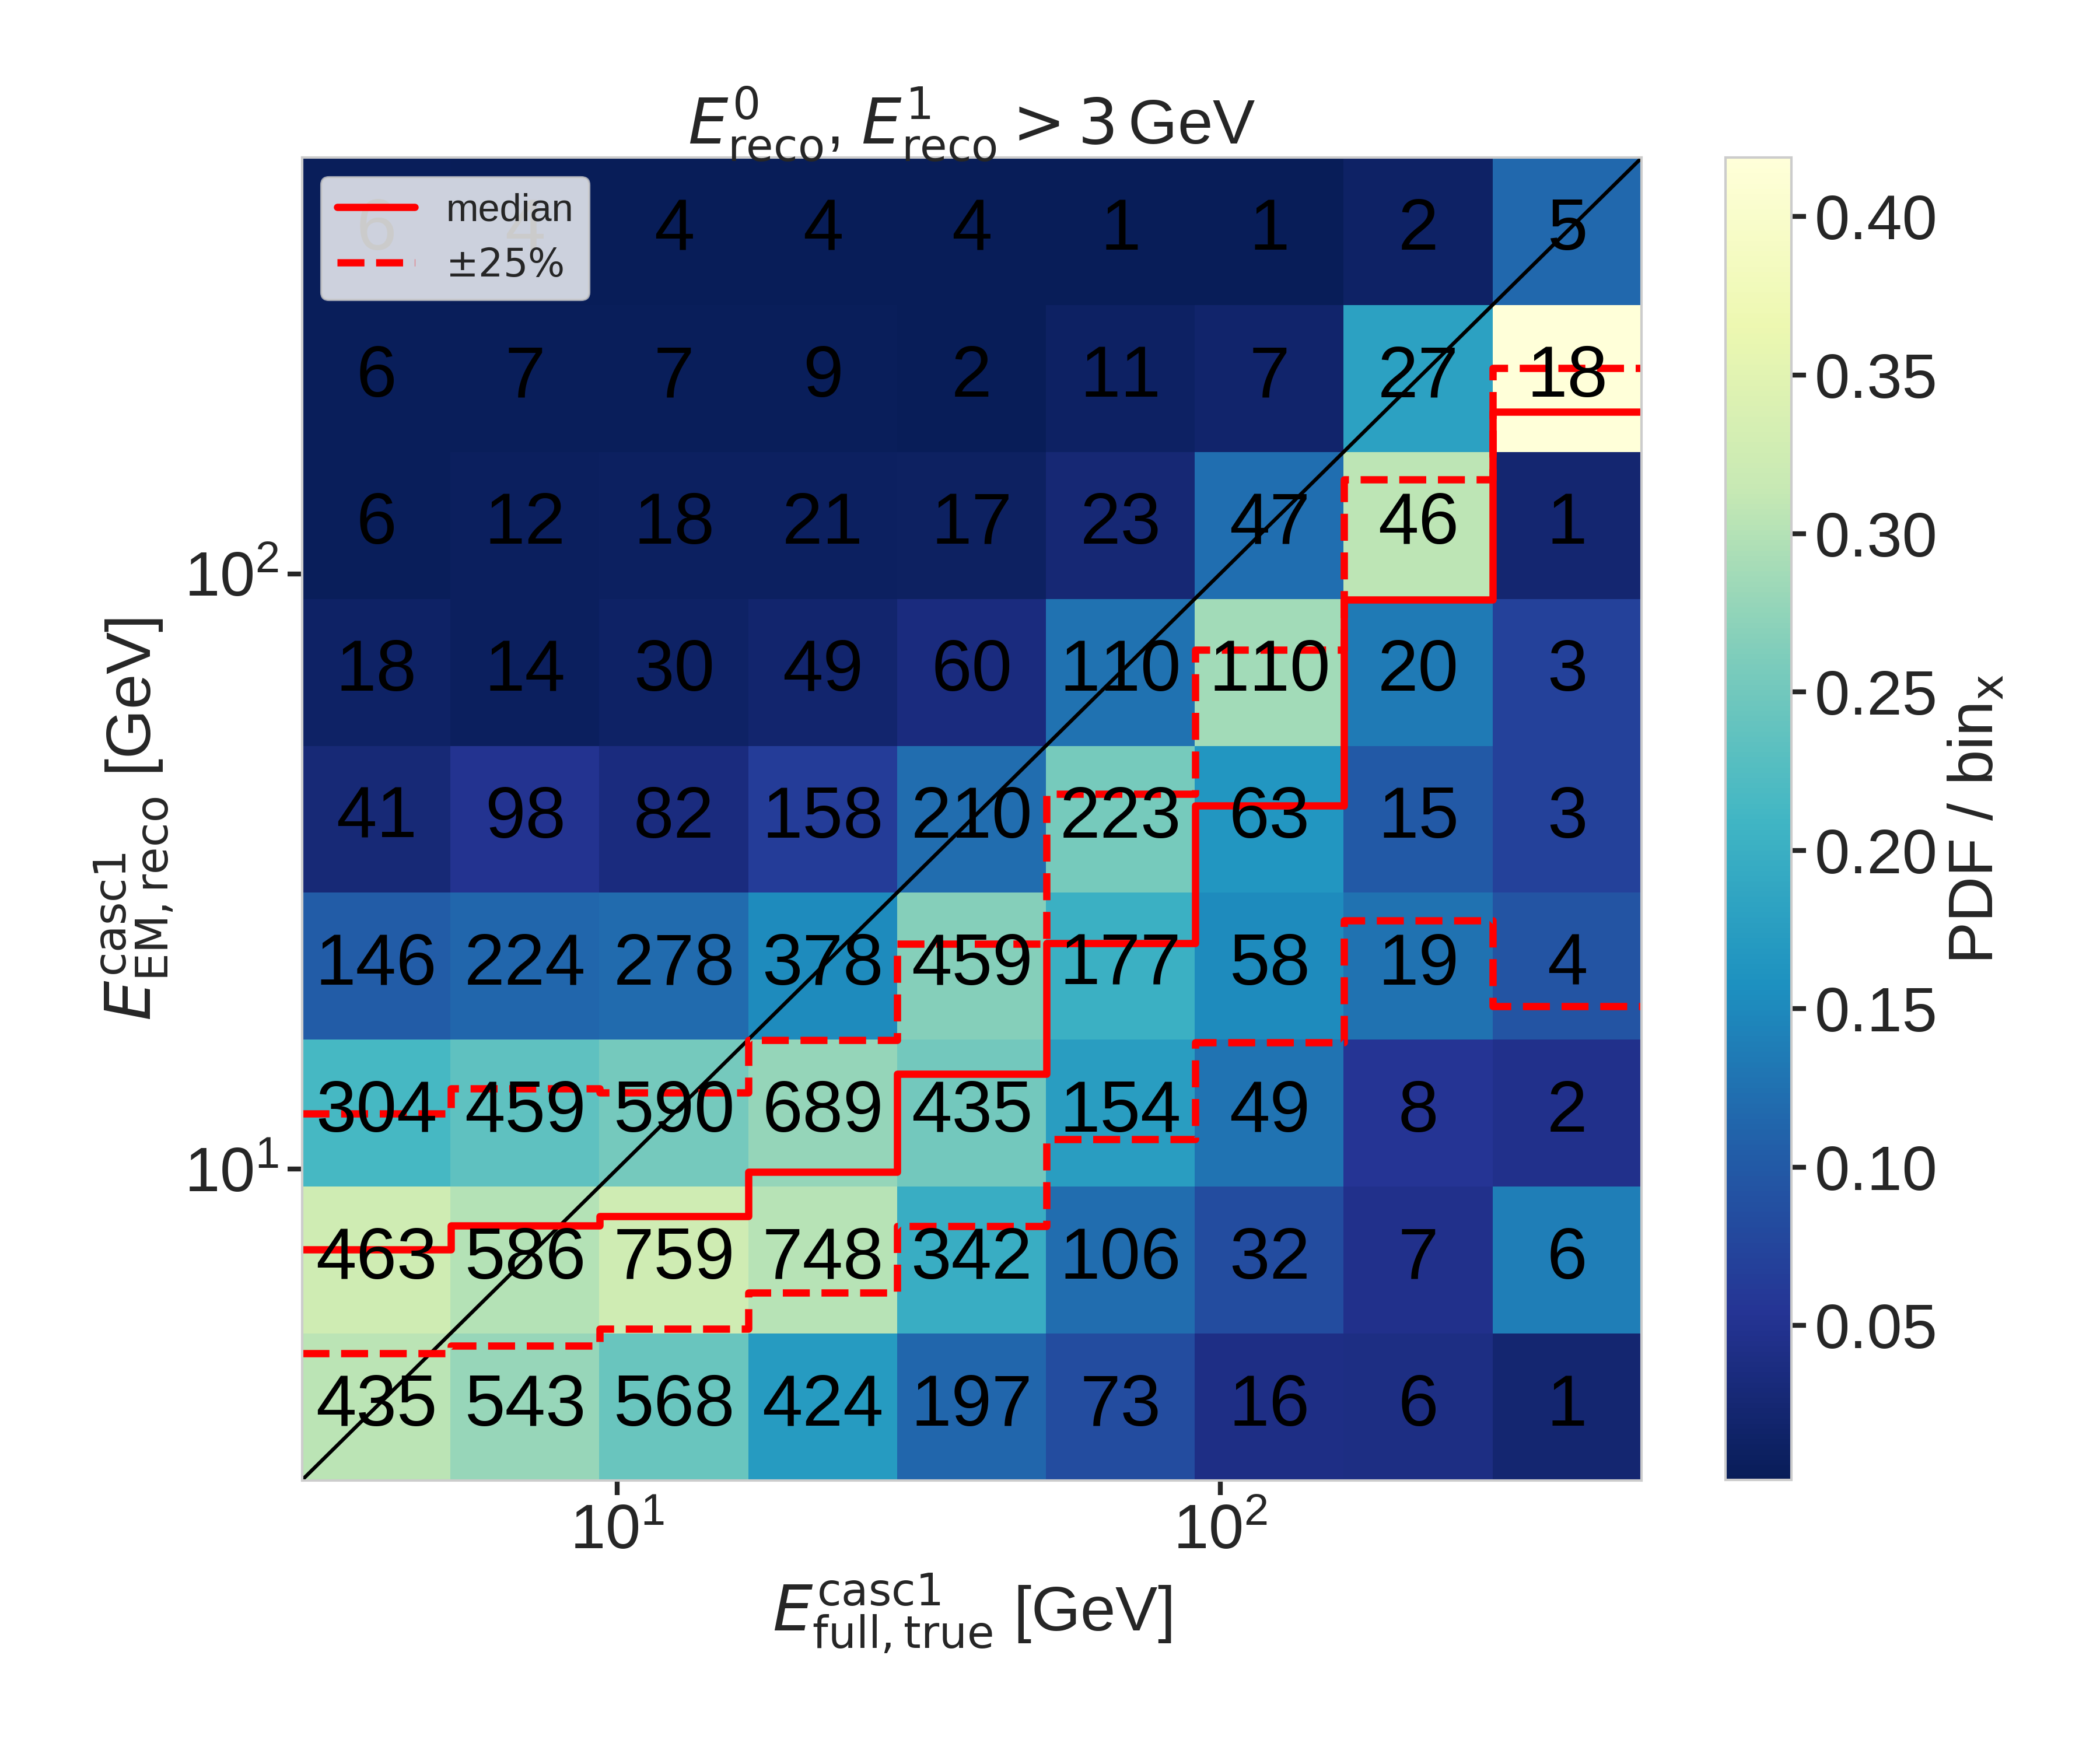
\includegraphics[width=0.49\linewidth]{figures/results/190605_reco_optimization/performance/selected_reco_chain_taupede_casc1_reco_energy_vs_casc1_true_energy_Good + L7 + reco E1,E2 above 3_step_contours.png}
    \caption[]{}
    \labfig{selected_routine_energy_results}
\end{figure*}
\todo{fix caption of this figure}


\section{Badly Reconstructed Cascade Population}

\paragraph{Ideas to write about:}
\begin{itemize}
    \item Show/highlight 2d decay length resolution again, basically 2 populations at higher energies
    \item only looking at events with >10 GeV instead of >3 GeV already improves the resolution a lot (low energy and therefore low light is a problem)
    \item take a closer look at those populations to find out what's going on
    \item multiple things were checked (bad direction (possibly due to seed), cascade position in DC, energies)
    \item the direction is worse for the badly reconstructed population, which could be due to a bad seed direction
    \item the events are a little further out radially, where the string/DOM spacing is not so tight, which also leads to less light being observed
    \item the energy of the second cascade is much lower than the first
    \item conclusion: it's a combination of all of them, but the main problem is the low energy
    \item true energies vs true length shows that first cascade energies are much larger than second (pick benchmark lengths and state the values!)
\end{itemize}


\section{Double Cascade Classification}

\paragraph{Missing Points}
\begin{itemize}
    \item MuMillipede "reconstruction" (depending on how deep I want to go into the classifier I tested?)
    \item This was done with the 190607 set (AFAIK), so I need to highlight what the differences are? 
    \item Calculated variables to input the classifier (distributions?)
    \item cuts applied to make sure the classifier is trained on well reconstructed events
    \item Tested classifier (BDT) versions and their performance
    \item takeaway
\end{itemize}

\section{Cross Checks}
\subsection{Simplistic Sets}

\todo{From HNL Note, re-write/change}

After generation the events are processed with standard Photon, Detector, L1, and L2 processing and then Taupede+MuMillipede is run on top of the L2 files. Multiple versions with different parameters were produced, some with the OscNext baseline parameters, some without detector noise (in Det level) and some with h2-50cm holeice model, to match the holeice model that was used to generate the photonics tables.


\paragraph{BrightDom Cleaning}

To investigate the effect of the BrightDom cleaning cut the 194601 set without detector noise (and baseline hole ice model) is used. The BrightDom cleaning is needed to stop a few DOMs with many photon hits to drive the reconstruction because this leads to large biases in the energy estimations. Historically, the BrightDom cleaning was removing all DOMs that had a charge larger than 10 times the mean charge. After quickly checking some charge distributions and how the mean behaves it was clear that the cut should better be defined based on a metric that is less affected by outliers, like the median. \reffig{bright_dom_cleaning_charges_mean_median} shows where the mean and the median are located for an example event. The cut was re-defined to use the median instead of the mean and 10\% of the simulation were processed with \href{https://github.com/LeanderFischer/I3_HNL_Decay/blob/a6838ec48e0a2d4f6547cbe064d2928ec55fb76d/submission_scripts/process/process_Taupede.py}{Taupede} using 30x and 100x the median as BrightDom cutoff. \reffig{bright_dom_cleaning_charges_median_scales} shows where these values fall for the same example event.

% \begin{figure}[h!]
%     \subfloat[\labfig{bright_dom_cleaning_charges_mean_median}]{
%         \includegraphics[width=.45\linewidth]{figures/upgoing_string_81_gen_level/brightdom_cleaning/median_and_mean_L2_00001.i3.zst_SplitInIcePulses_frame_0.png}
%         }
%     \subfloat[\labfig{bright_dom_cleaning_charges_median_scales}]{
%         \includegraphics[width=.45\linewidth]{figures/upgoing_string_81_gen_level/brightdom_cleaning/median_scales_L2_00001.i3.zst_SplitInIcePulses_frame_0.png}
%         }
%     \caption{Charge distribution of example event showing mean and median charge (left) and different scales of median charge (right).}
%     \labfig{bright_dom_cleaning_charges}
% \end{figure}

As a quick check of the performance of both cuts the decay length resolution/bias and the resolutions/biases of all energies were checked. The reconstructed decay length is almost not affected by applying this cut, which is as expected, because it is mostly dependent on the arrival time of the photons. The effect on the reconstructed energy is much stronger, where a looser cut (100x) shows a significantly larger bias than the tighter cut at (30x). Even though this was not a highly sophisticated optimization of the BrightDom cut, an improvement was achieved by changing from mean to median and selecting the tighter cut (of the two tested). It's hard to tell how this would perform for high energy events, but I'm quite certain that a definition based on the median would be more reliable than on the mean.

% \begin{figure}[h!]
%     \subfloat[\labfig{bright_dom_cleaning_performance_decay_length_bias}]{
%         \includegraphics[width=.45\linewidth]{figures/upgoing_string_81_gen_level/brightdom_cleaning/median_decay_length_bias_fullset_larger_range_unweighted.png}
%         }
%     \subfloat[\labfig{bright_dom_cleaning_performance_total_energy_bias}]{
%         \includegraphics[width=.45\linewidth]{figures/upgoing_string_81_gen_level/brightdom_cleaning/compare_bright_dom_cuts_fractional_reco_total_energy_error_fully.png}
%         }
%     \caption{Decay length bias (left) and total energy bias (right).}
%     \labfig{bright_dom_cleaning_performance}
% \end{figure}

\section{Performance}

\subsection{Energy/Decay Length Resolution}

\todo{describe the "good fit" selection}

\subsubsection{2-D Histograms}

\textbf{Things to mention about the 2d-hists:}
\begin{itemize}
    \item total energy resolution looks very good, above \SI{10}{\gev} it's almost unbiased and the 1-sigma resolution band is below \SI{20}{\percent}
    \item individual cascade resolutions mirror this behavior, but are starting to stabilize in energy at lower energies around \SIrange{5}{6}{\gev} with a broader resolution band of \SI{50}{\percent}, but reducing drastically with increasing energy (down to \SI{20}{\percent} at \SI{100}{\gev})
    \item interestingly, the second cascade energy reconstruction performs slightly worse, although they have the same energy ranges. This could hint at an asymmetry in the reconstruction process (might relate to how the two cascades are parameterized) or be due to the different positions and the dominantly up-going direction used in the sampling combined with the DOMs looking down (relate this to the sampling distribuitons explained/shown in the previous chapter)
    \item the decay length resolution looks much worse. In the region between \SIrange[range-phrase={~and~}]{20}{80}{\meter} it's roughly unbiased, but 1-sigma resolution band is quite wide with a lot of outliers towards short reconstructed lengths. Below \SI{20}{\meter} the reconstructed lengths are always over-estimating the true and above \SI{80}{\meter} a population of events start to dominate where the decay lengths isn't getting reconstructed at all, which might indicate that one of the cascades wasn't observers. (Relate to the fact that this marginalizes over all energies, meaning also all events which have one cascade with very low energy are included here.)
    \item another interesting feature is the band of reconstructed lengths around \SI{100}{\meter}, which is probabaly related to the spacing between most of the strings, which favors the reconstruction to be around this value, because that's the distance at which light can be observed, just from the fact that the DOMs are spaced at this distance (for low energetic cascades, this can dominate the reconstruction)
\end{itemize}


\begin{figure*}[h]
	\centering
    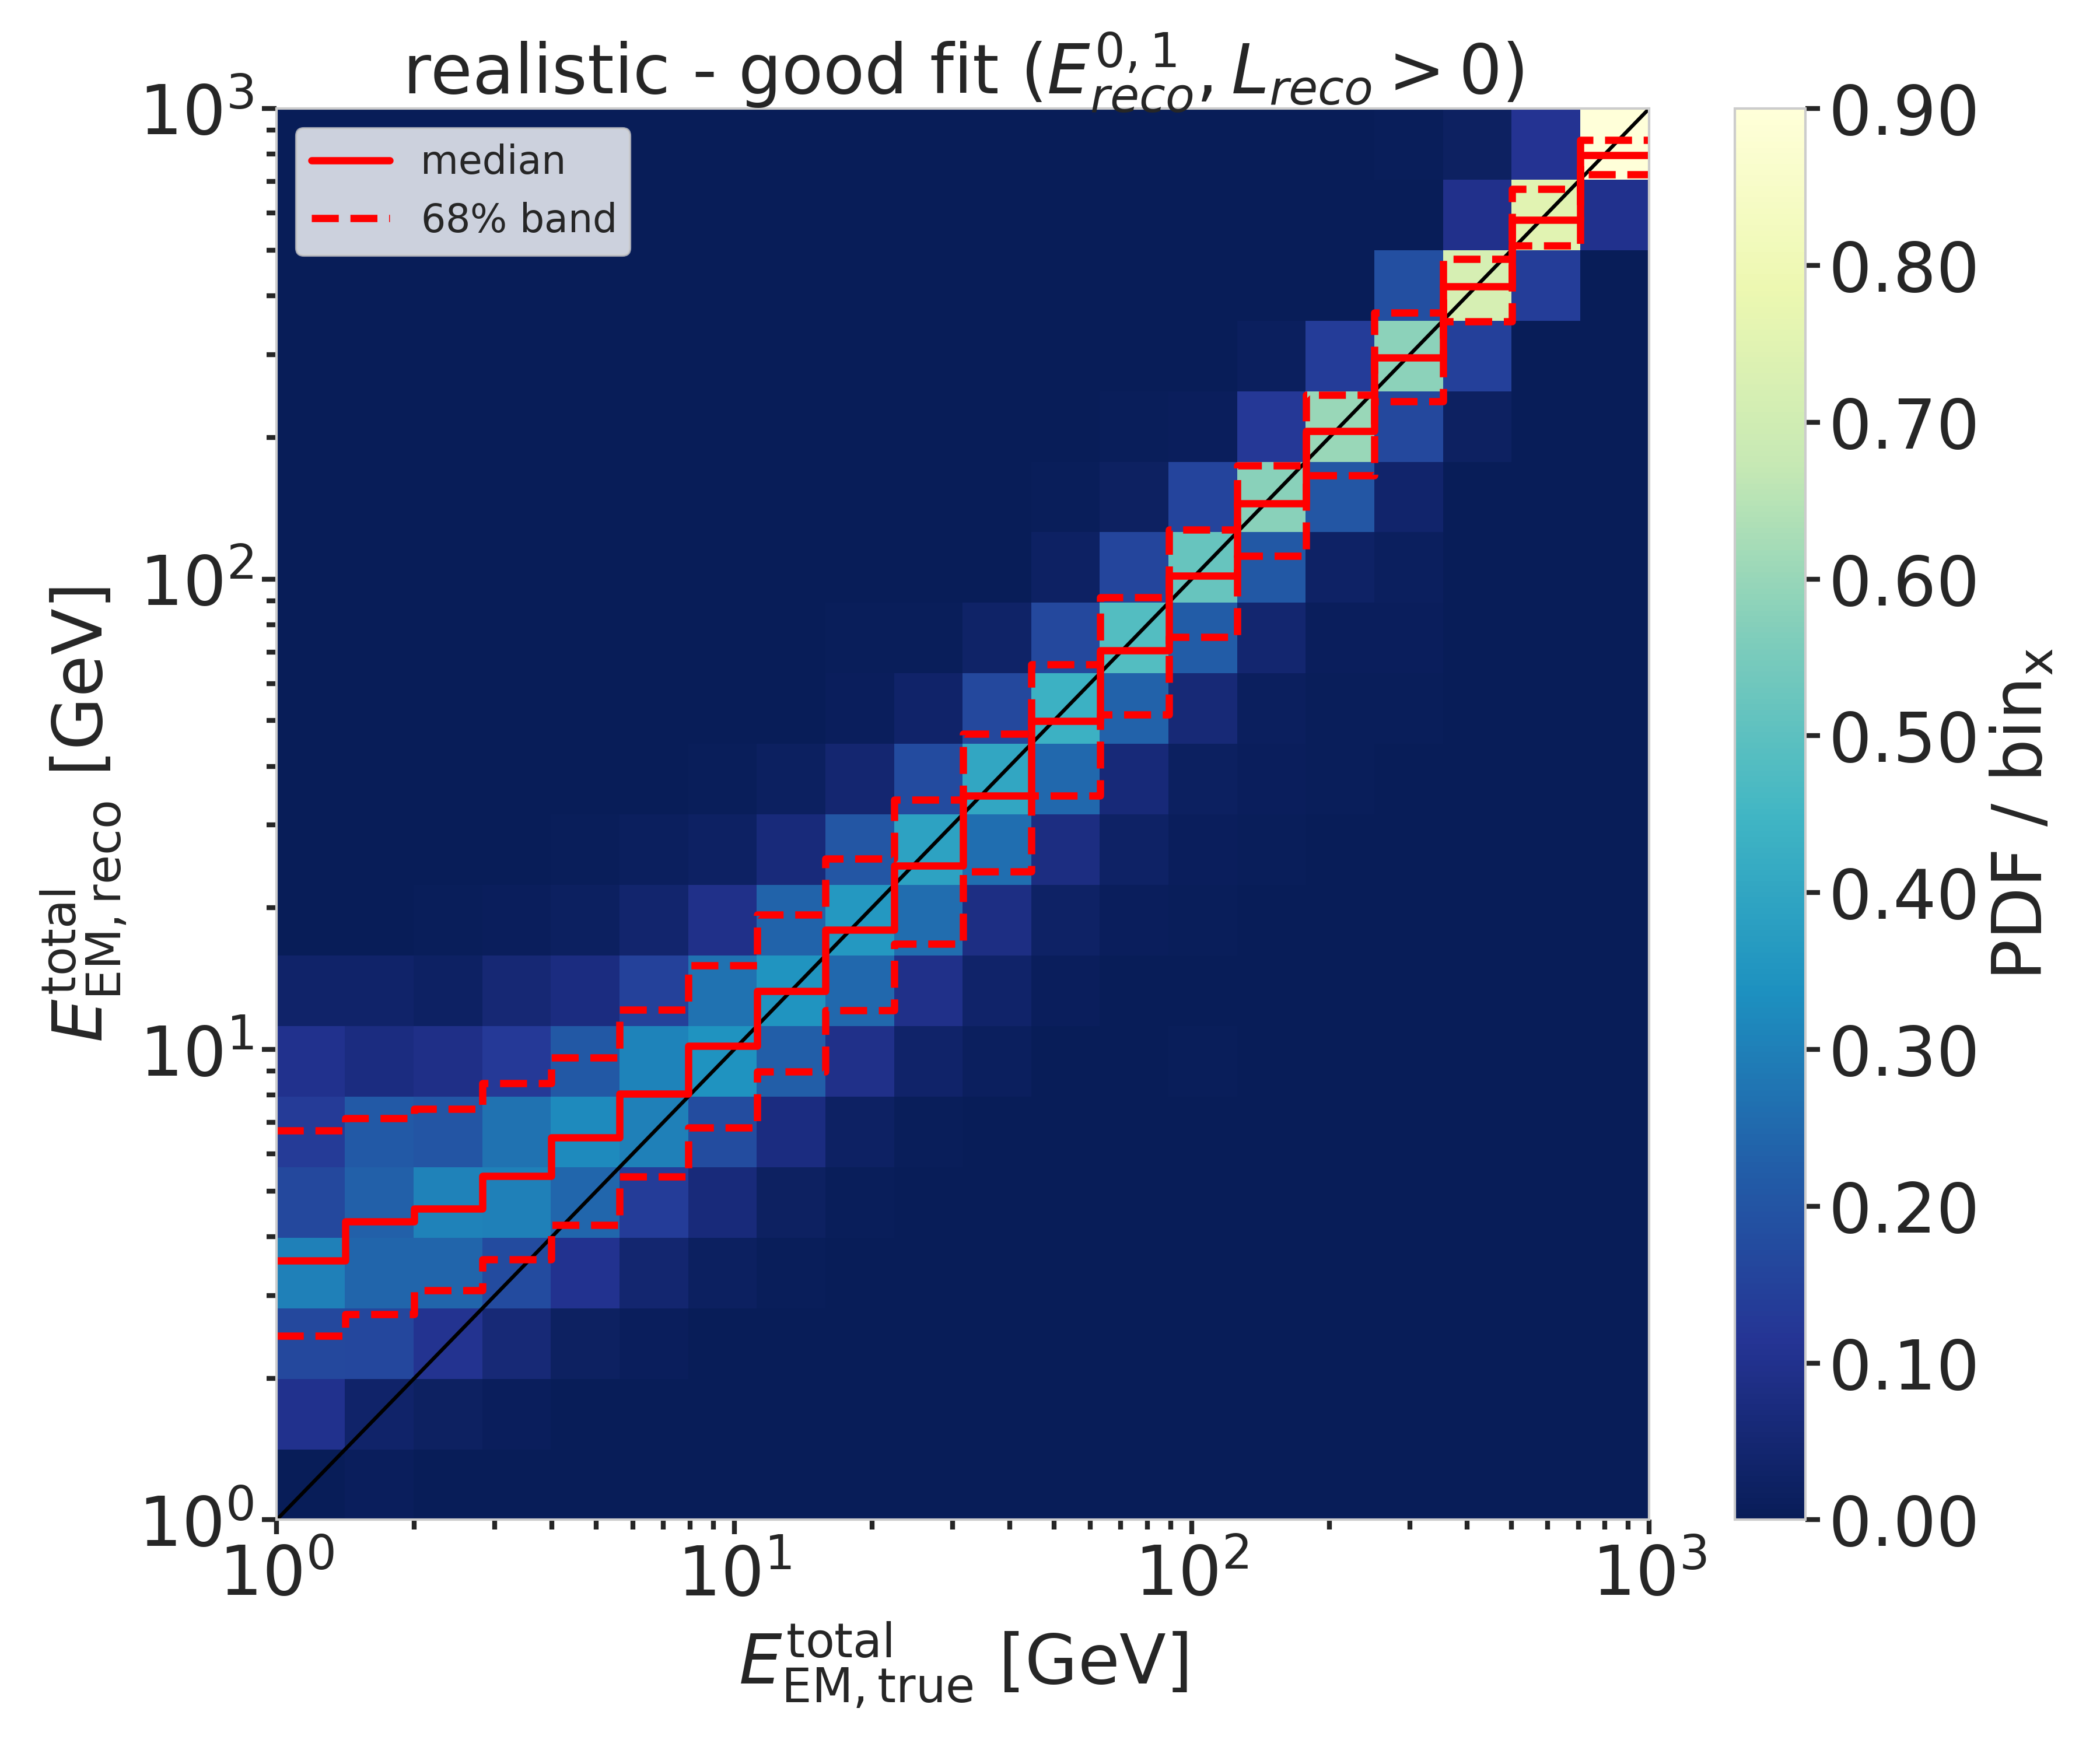
\includegraphics[width=0.49\linewidth]{figures/model_independent_simulation/results/realistic/2d_hists/194603_reco_total_energy_vs_true_total_energy_goodfit_step_contours.png}
    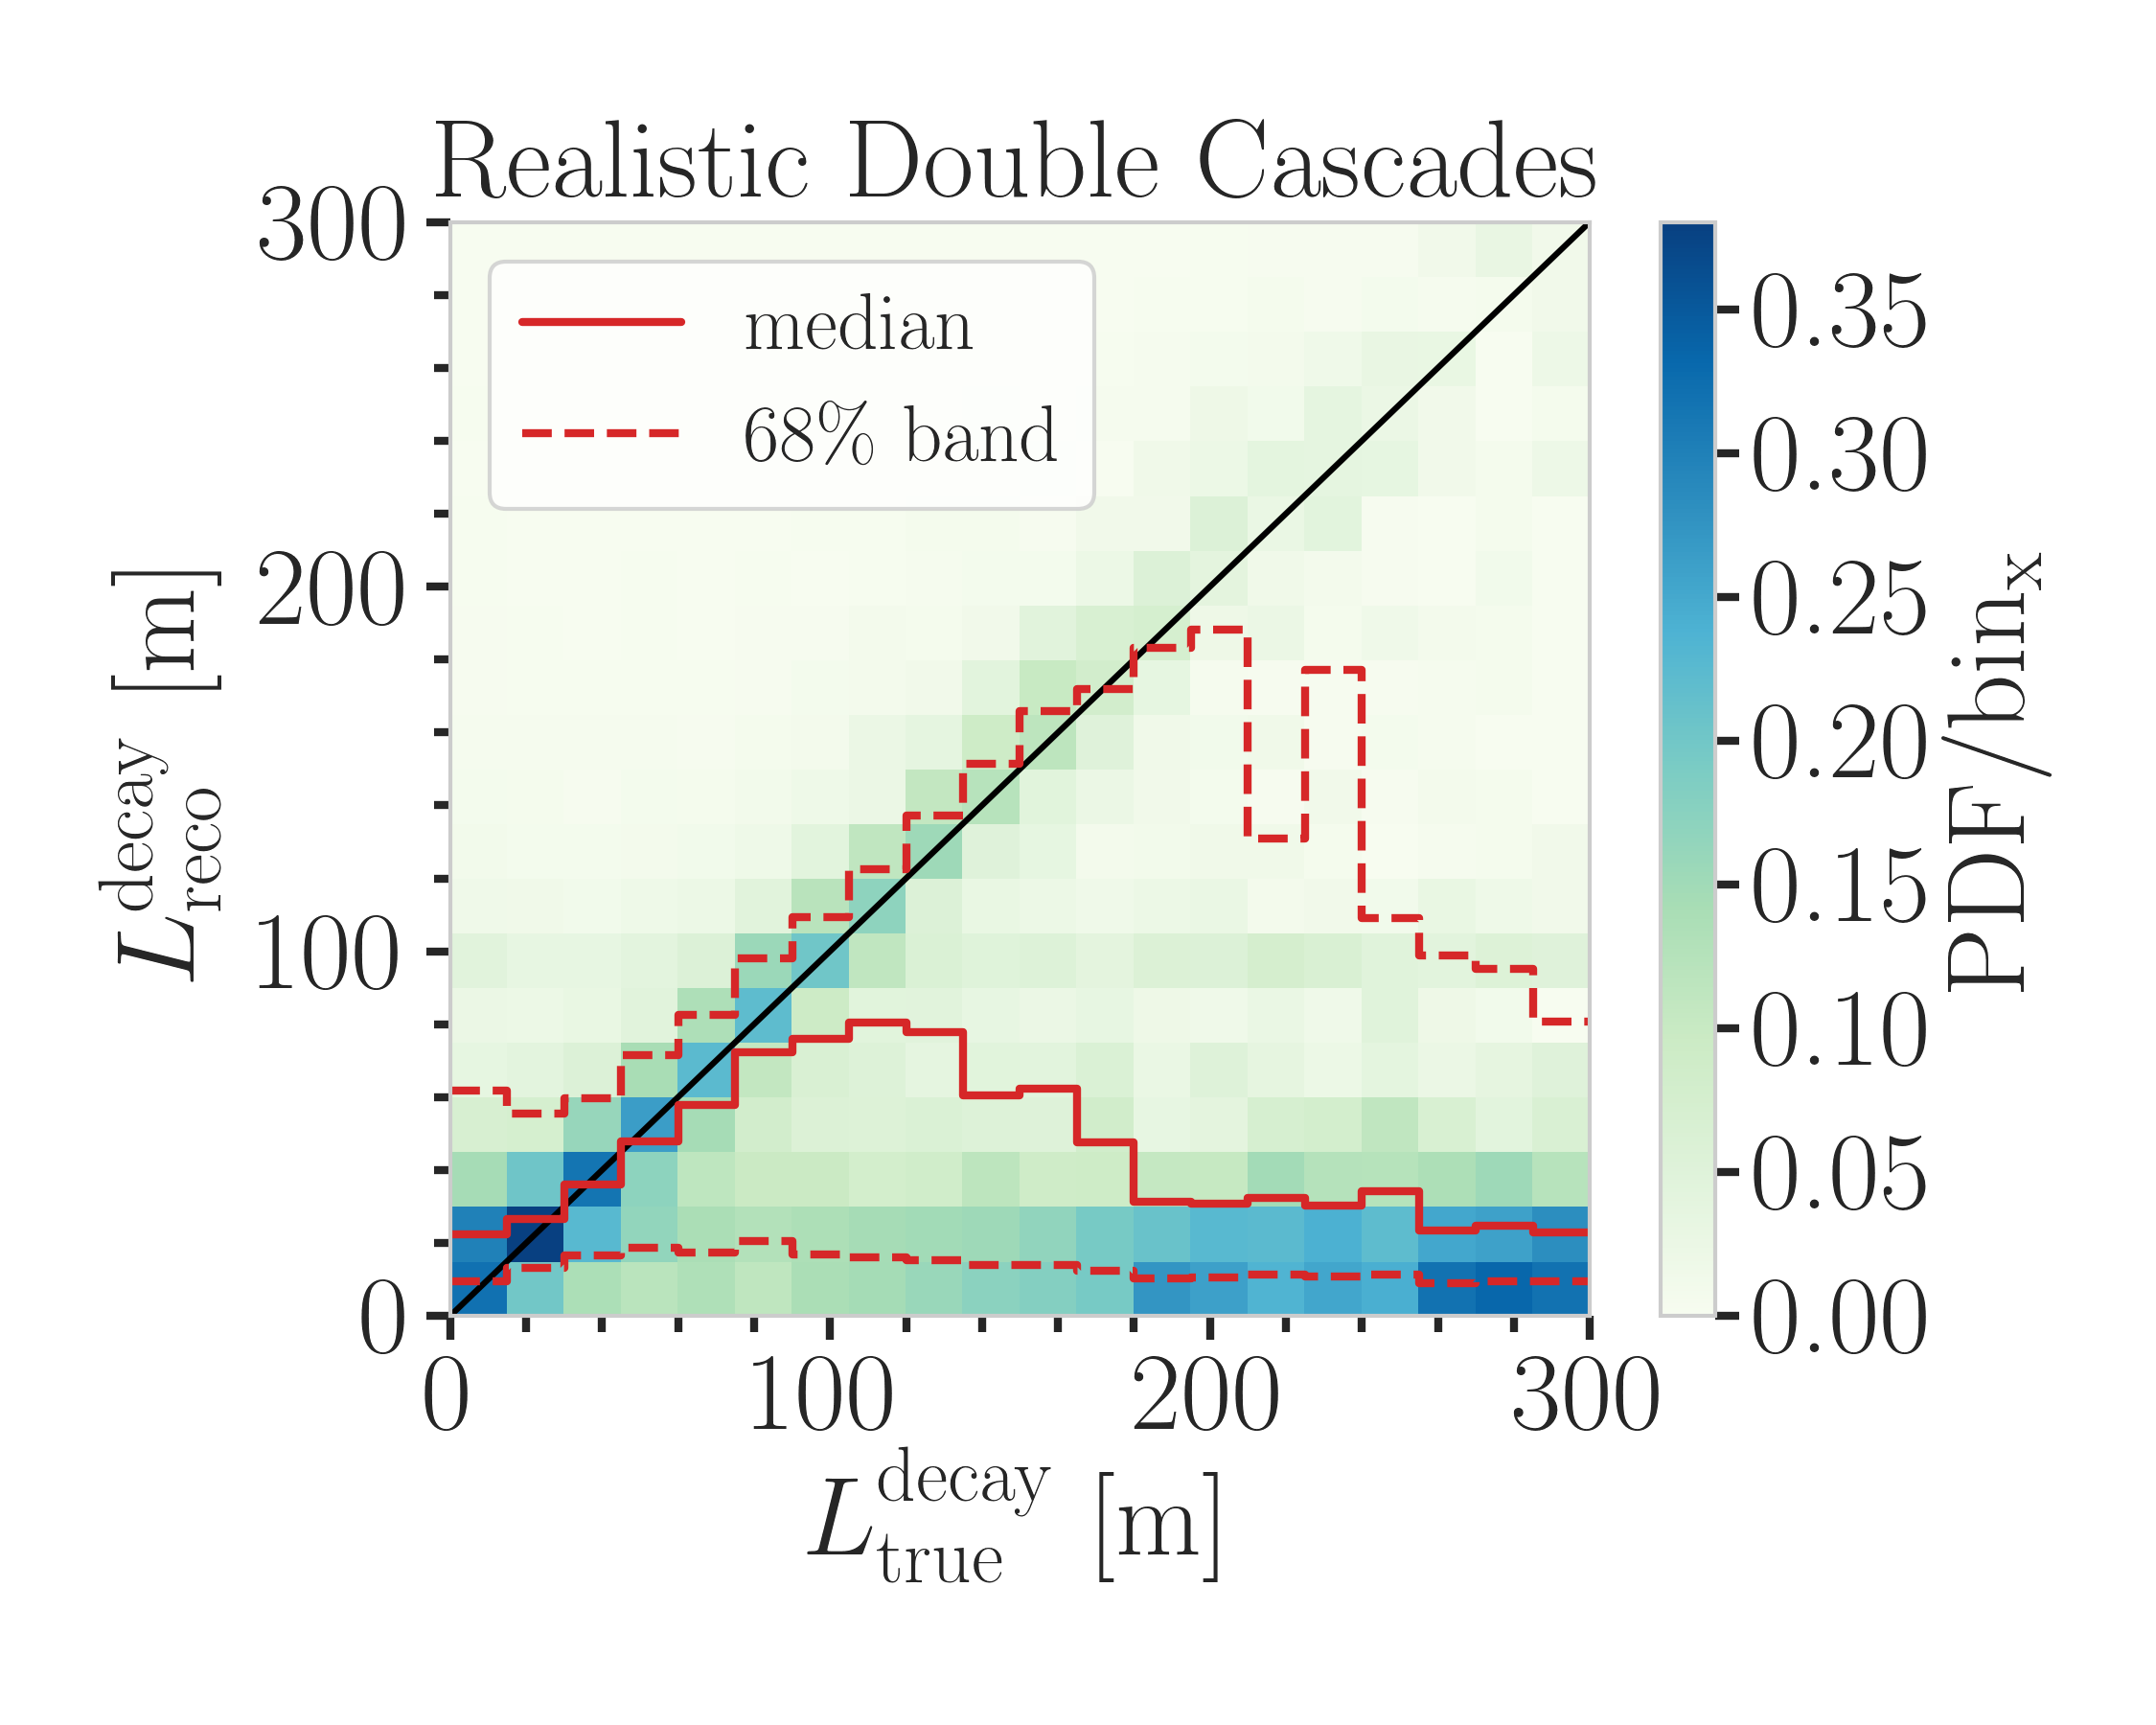
\includegraphics[width=0.49\linewidth]{figures/model_independent_simulation/results/realistic/2d_hists/194603_reco_decay_length_vs_true_decay_length_goodfit_step_contours.png}
    \caption[]{}
    \labfig{total_energy_decay_length_2dhists}
\end{figure*}

\begin{figure*}[h]
	\centering
    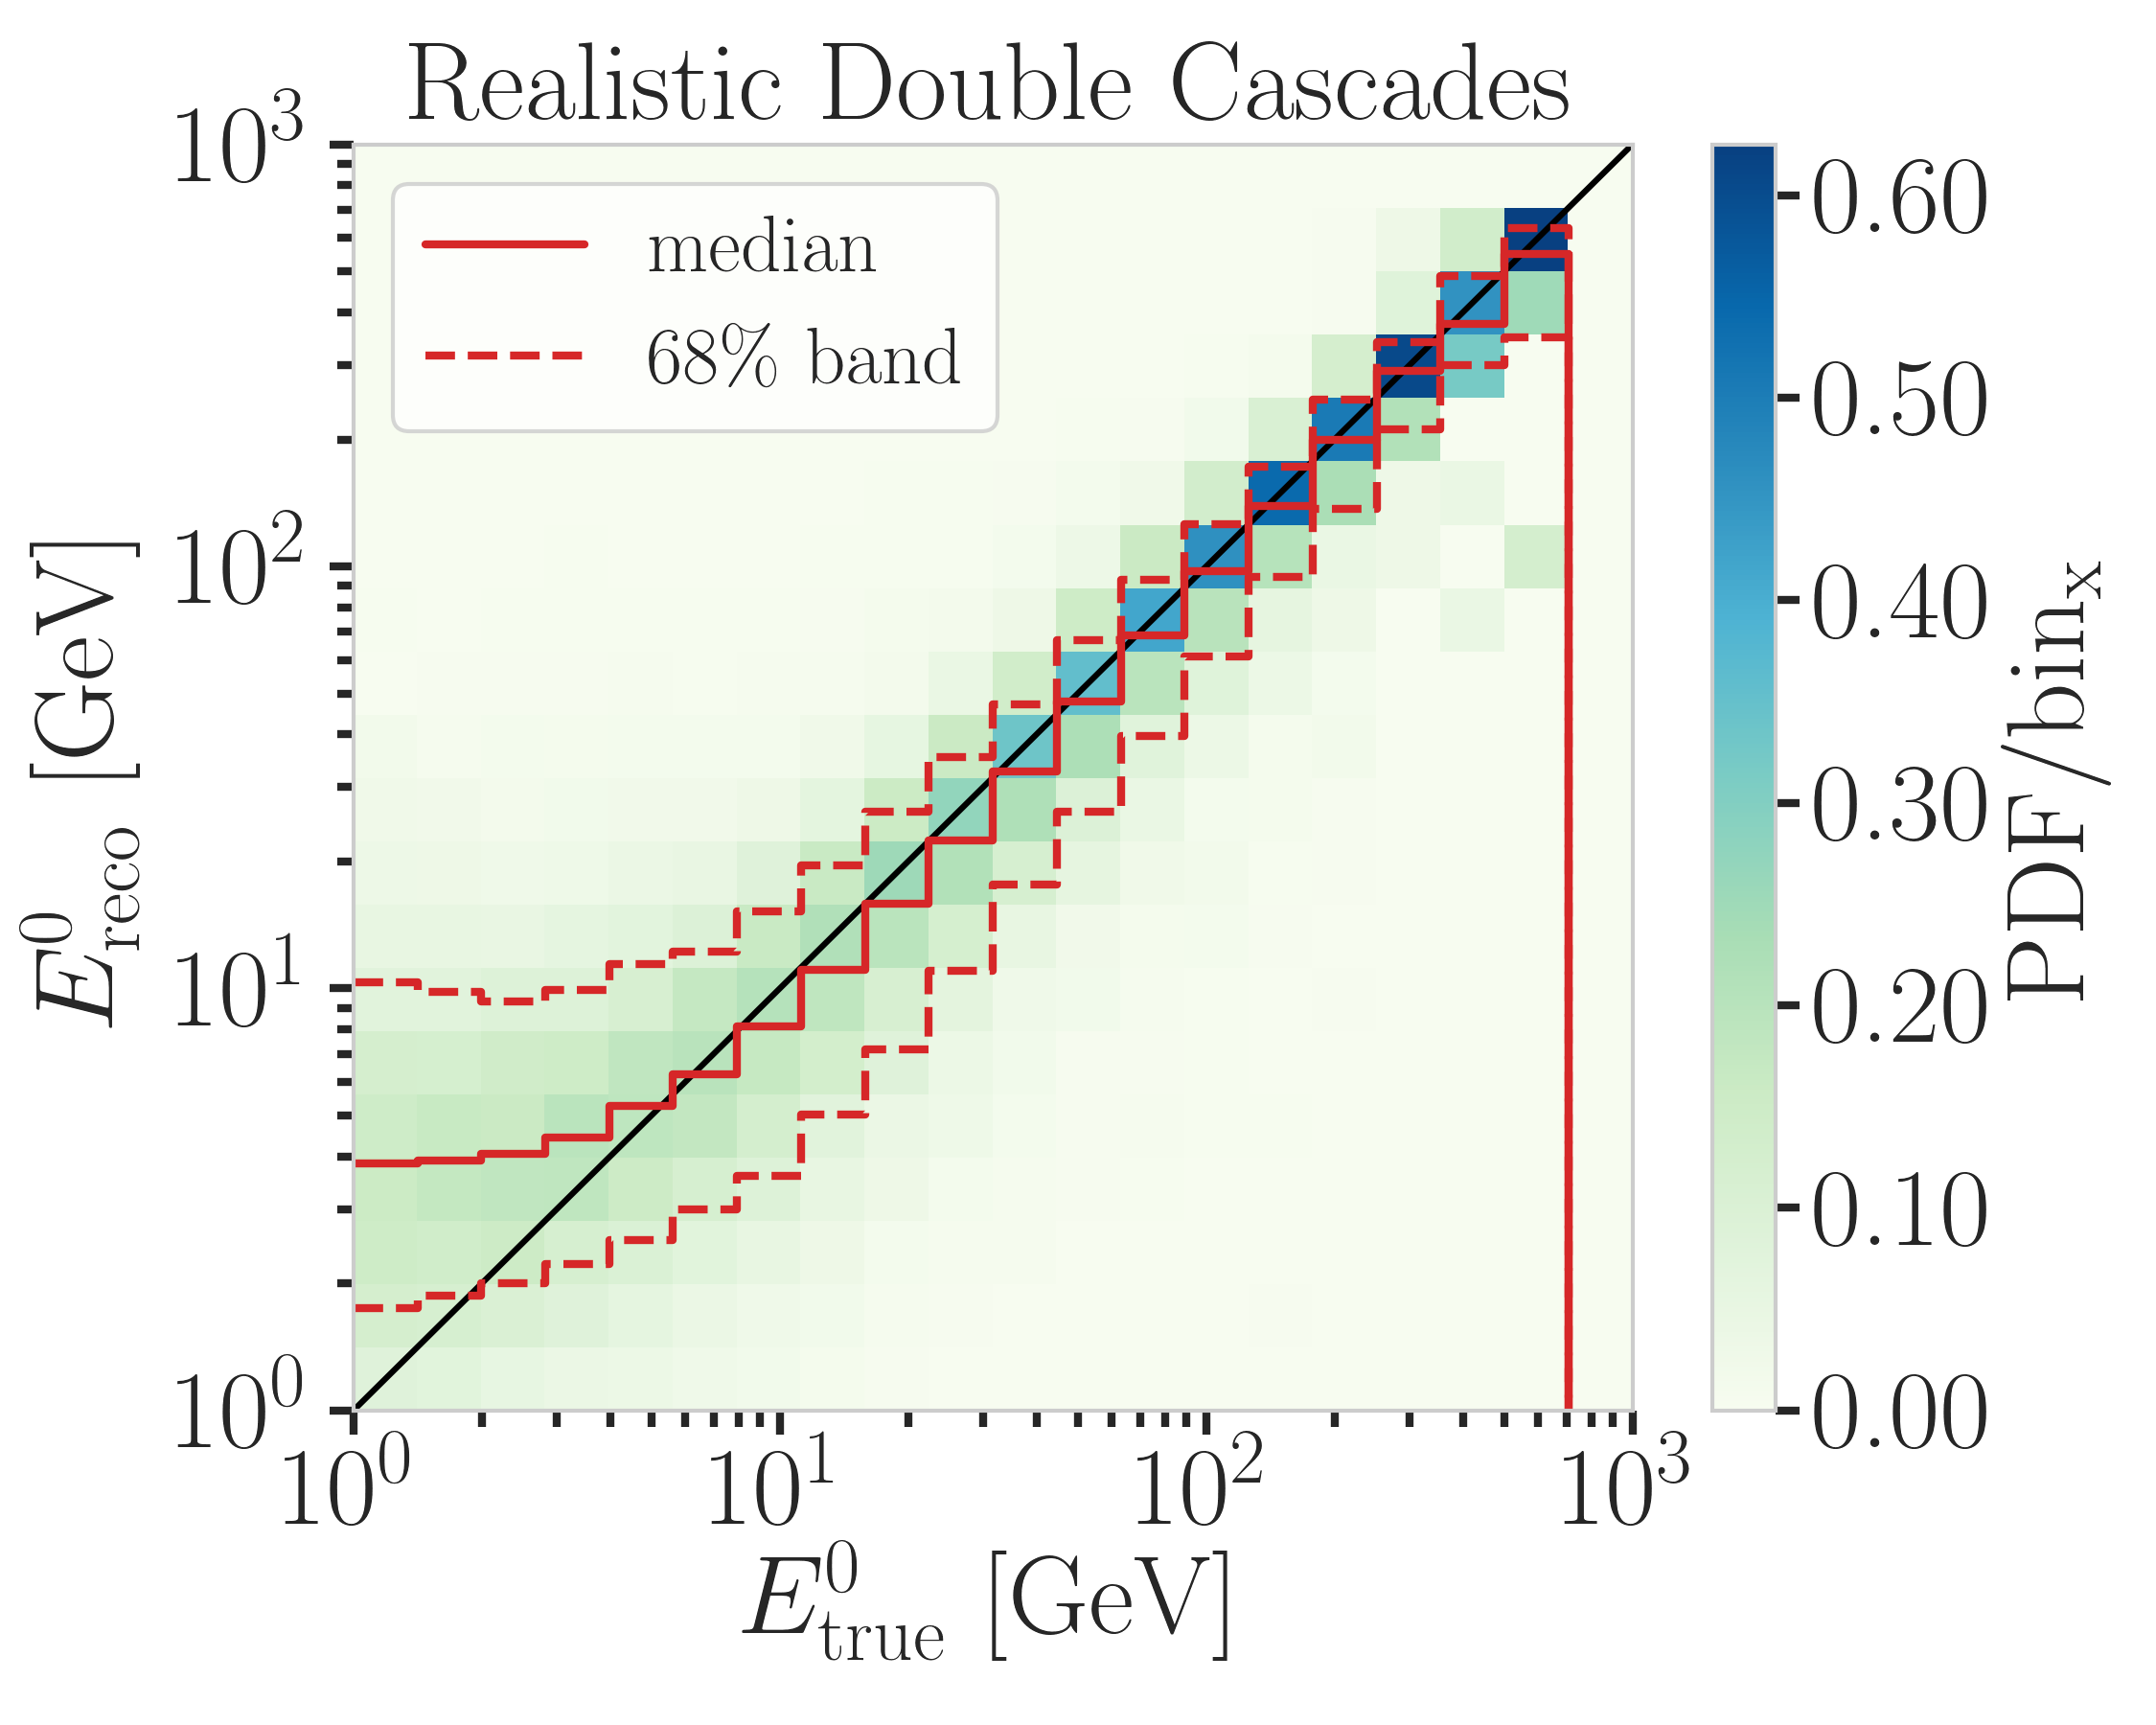
\includegraphics[width=0.49\linewidth]{figures/model_independent_simulation/results/realistic/2d_hists/194603_casc0_reco_energy_vs_casc0_true_energy_goodfit_step_contours.png}
    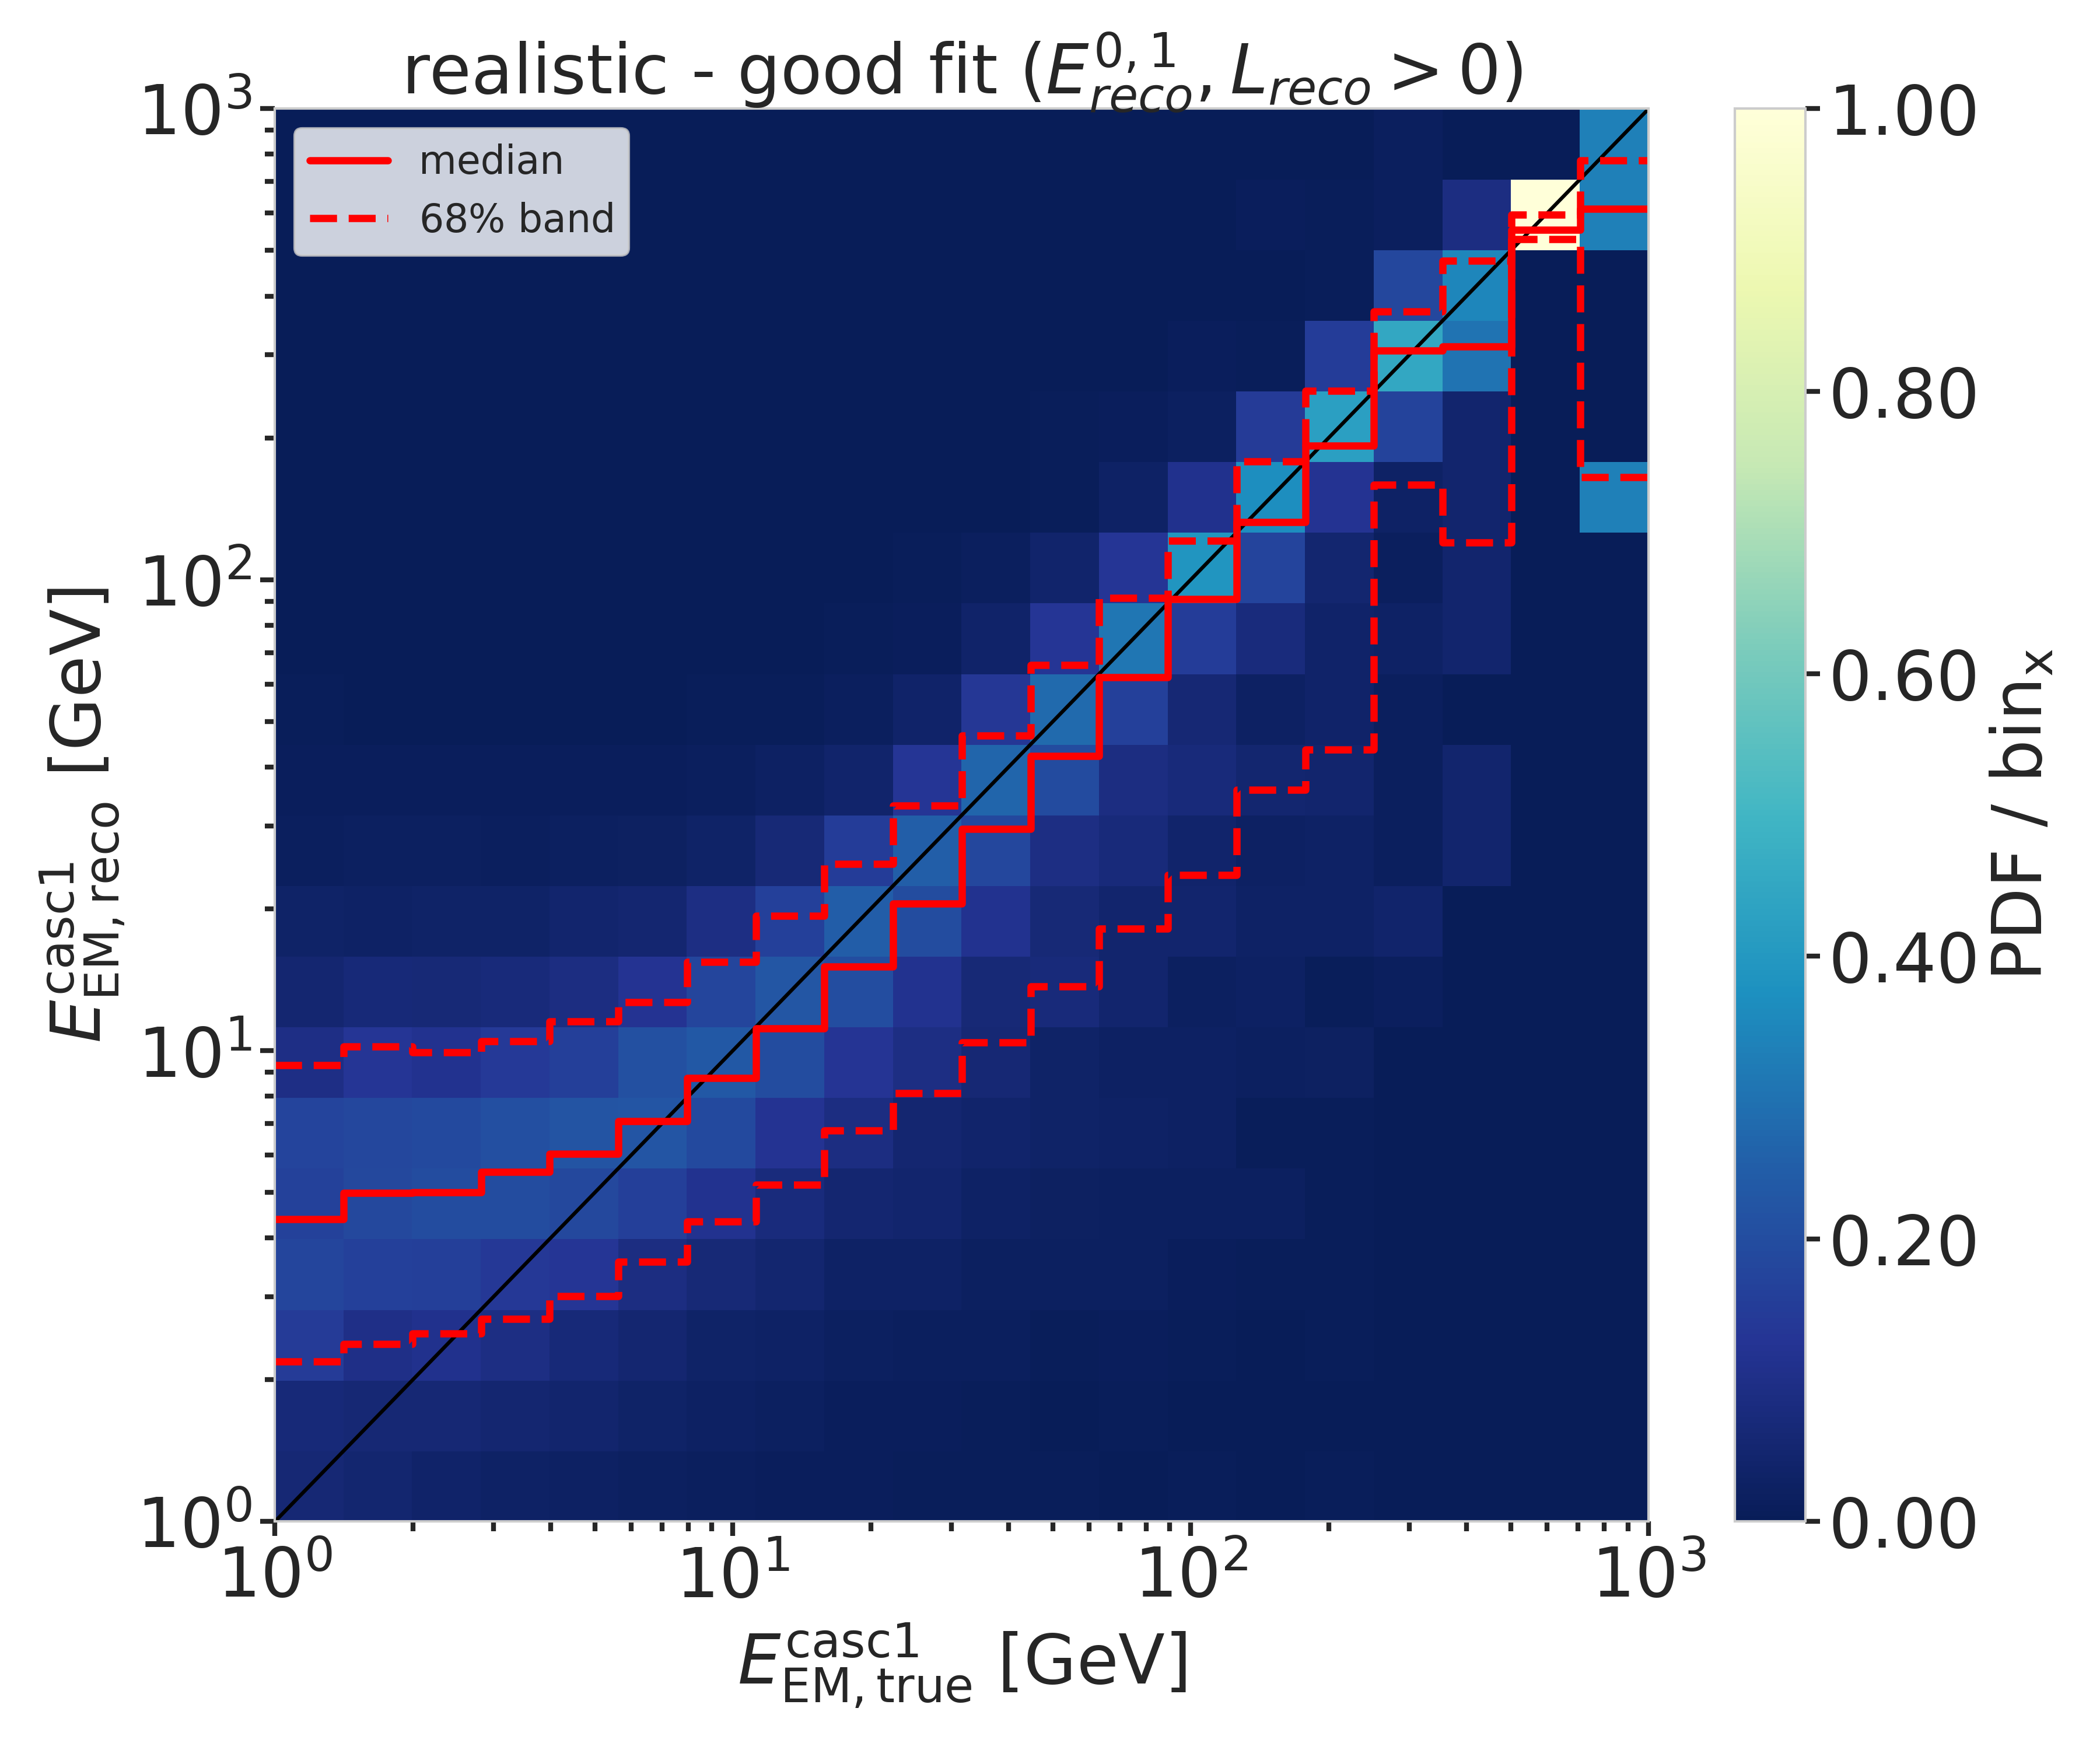
\includegraphics[width=0.49\linewidth]{figures/model_independent_simulation/results/realistic/2d_hists/194603_casc1_reco_energy_vs_casc1_true_energy_goodfit_step_contours.png}
    \caption[]{}
    \labfig{cascade_energy_2dhists}
\end{figure*}


\subsubsection{Energy Resolution}

\textbf{Things to mention about the energy resolution:}
\begin{itemize}
    \item Here it can be seen more clearly how the median total energy resolution starts to stabilize around 0.0 at \SI{10}{\gev}, while for lower energies the reconstruction is over-estimating the true energy. This is a known behavior of energy reconstructions in IceCube, which is mainly due to a selection effect. Only events with a certain amount of light can be reconstructed, which means that the ones with true small energies that are still in the sample are events with over average light production due to fluctuations or other effects?
\end{itemize}

\begin{figure}[h]
	\centering
    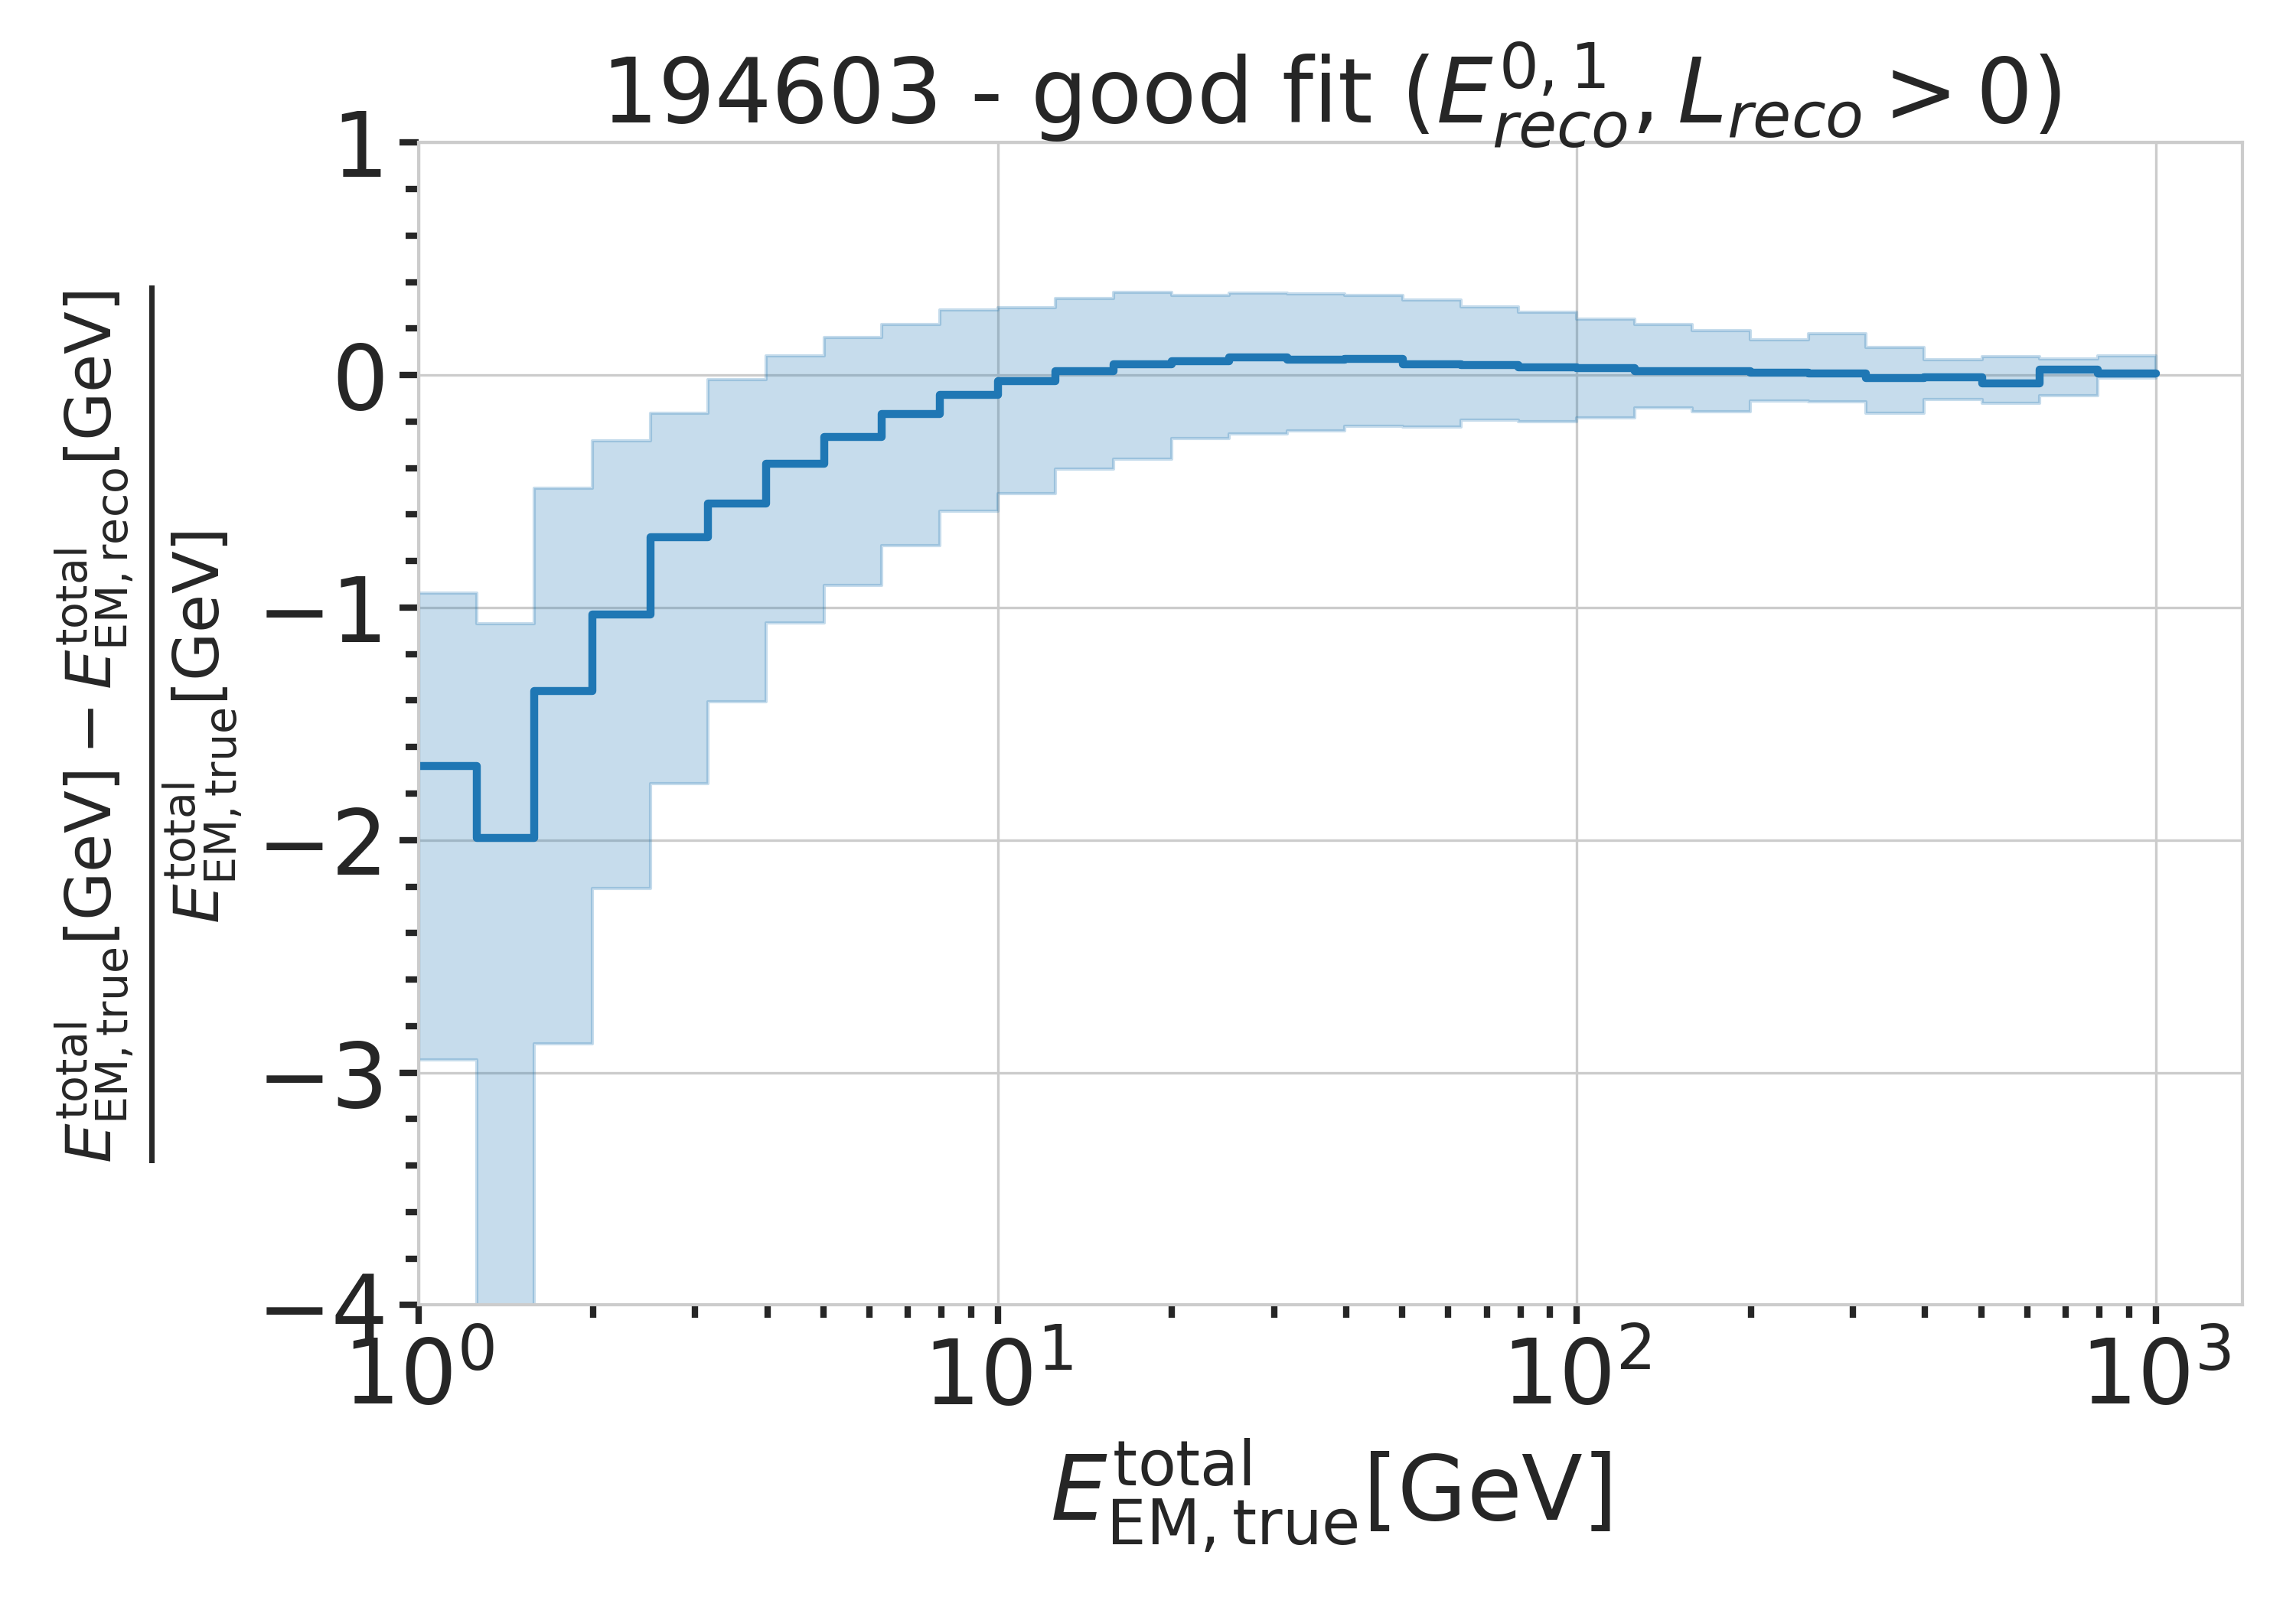
\includegraphics{figures/model_independent_simulation/results/realistic/resolutions/194603_fractional_reco_total_energy_error_goodfit.png}
    \caption[]{}
    \labfig{total_energy_bias_vs_energy}
\end{figure}


\subsubsection{Decay Length Resolution}

\textbf{Things to mention about the decay length resolution:}
\begin{itemize}
    \item As already mentioned before, the decay length resolution is much worse than the energy resolutions. \reffig{decay_length_bias_vs_length} also shows that the median is below 0.0 for short true length and above 0.0 and approaching 1.0 for long true lengths.
    \item To investigate whether this is really due to the fact that one of the cascades is not observed, the decay length resolution was plotted against the total energy of the event and the minimum energy of the two cascades \reffig{decay_length_bias_vs_energies}.
    \item It can be seen that the median of the decay length resolution stabilizes at 0.0 for a total energy above \SI{20}{\gev}, but the spread of the distribution is still quite large with a 1-sigma band of \SIrange{80}{100}{\percent}.
    \item From the plot against the minimum energy it can be seen that the decay length resolution starts to be unbiased for a minimum energy of the cascades of \SI{7}{\gev}, with an equivalently large spread.
    \item A preliminary takeaway from this is that the decay length reconstruction is not reliable at all for events with a total energy below \SI{20}{\gev} or a minimum cascade energy below \SI{7}{\gev}.
\end{itemize}

\begin{figure}[h]
	\centering
    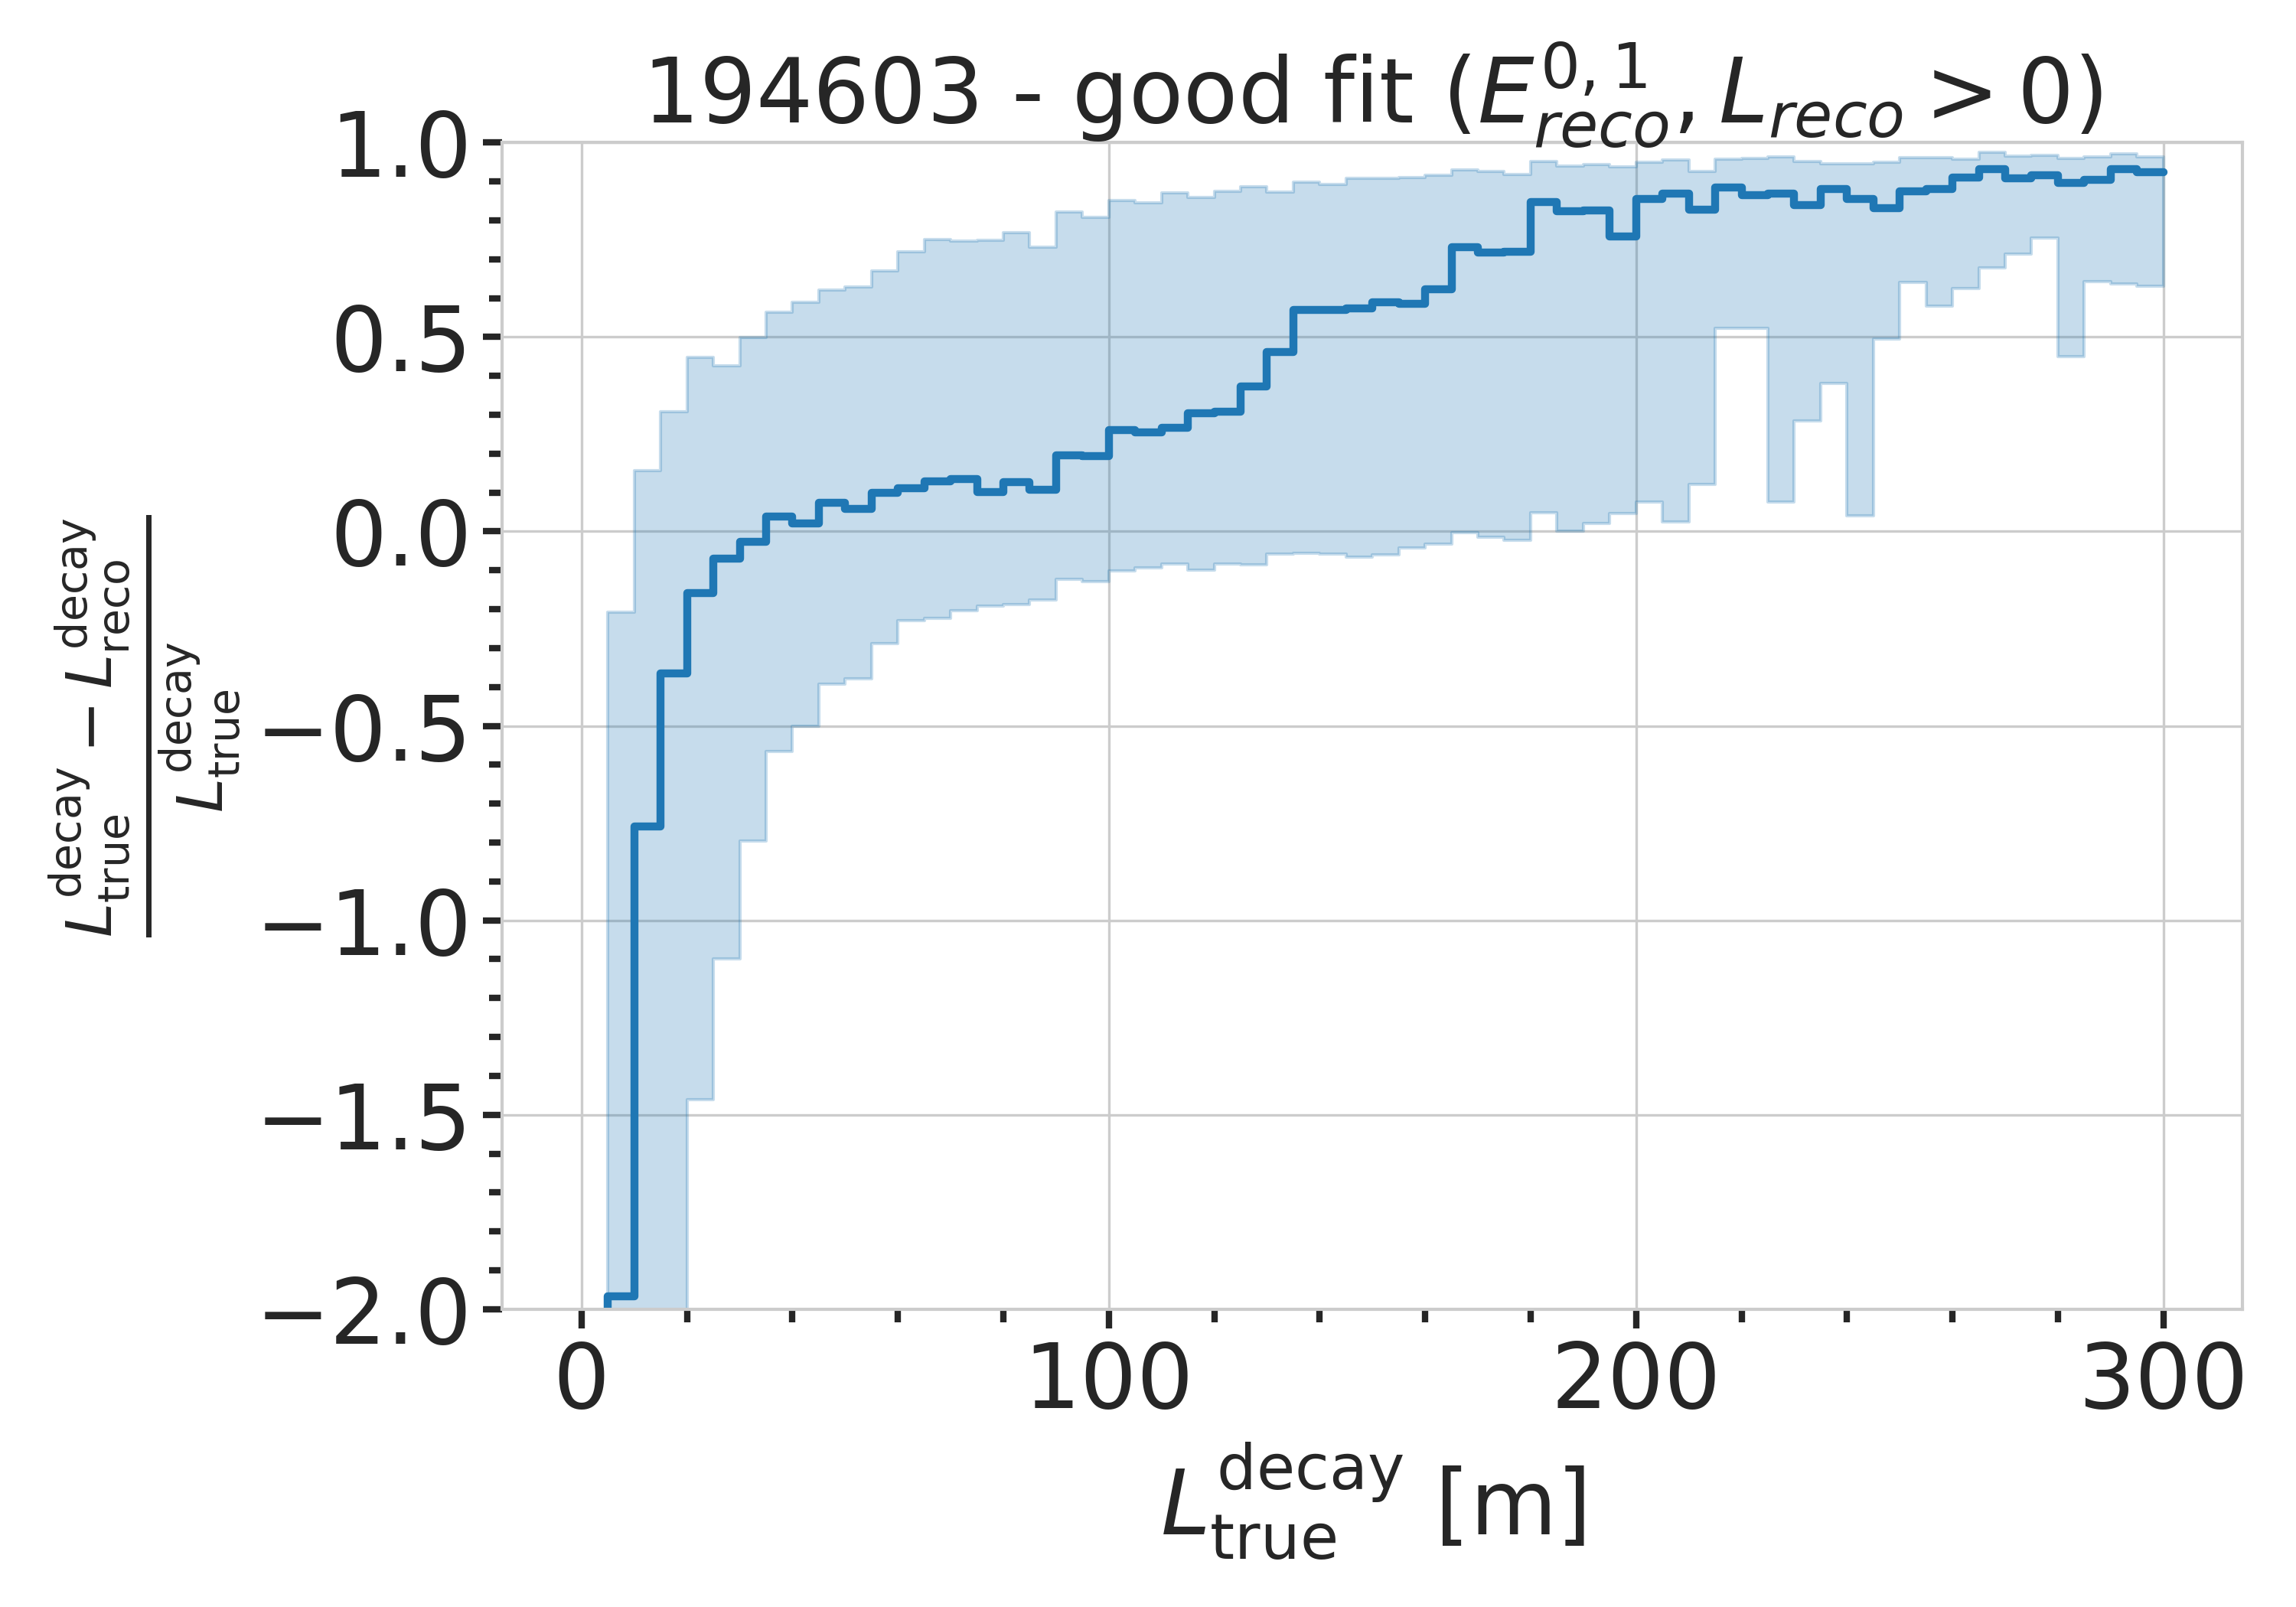
\includegraphics{figures/model_independent_simulation/results/realistic/resolutions/194603_median_decay_length_bias_goodfit_log_unweighted.png}
    \caption[]{}
    \labfig{decay_length_bias_vs_length}
\end{figure}


\begin{figure*}[h]
	\centering
    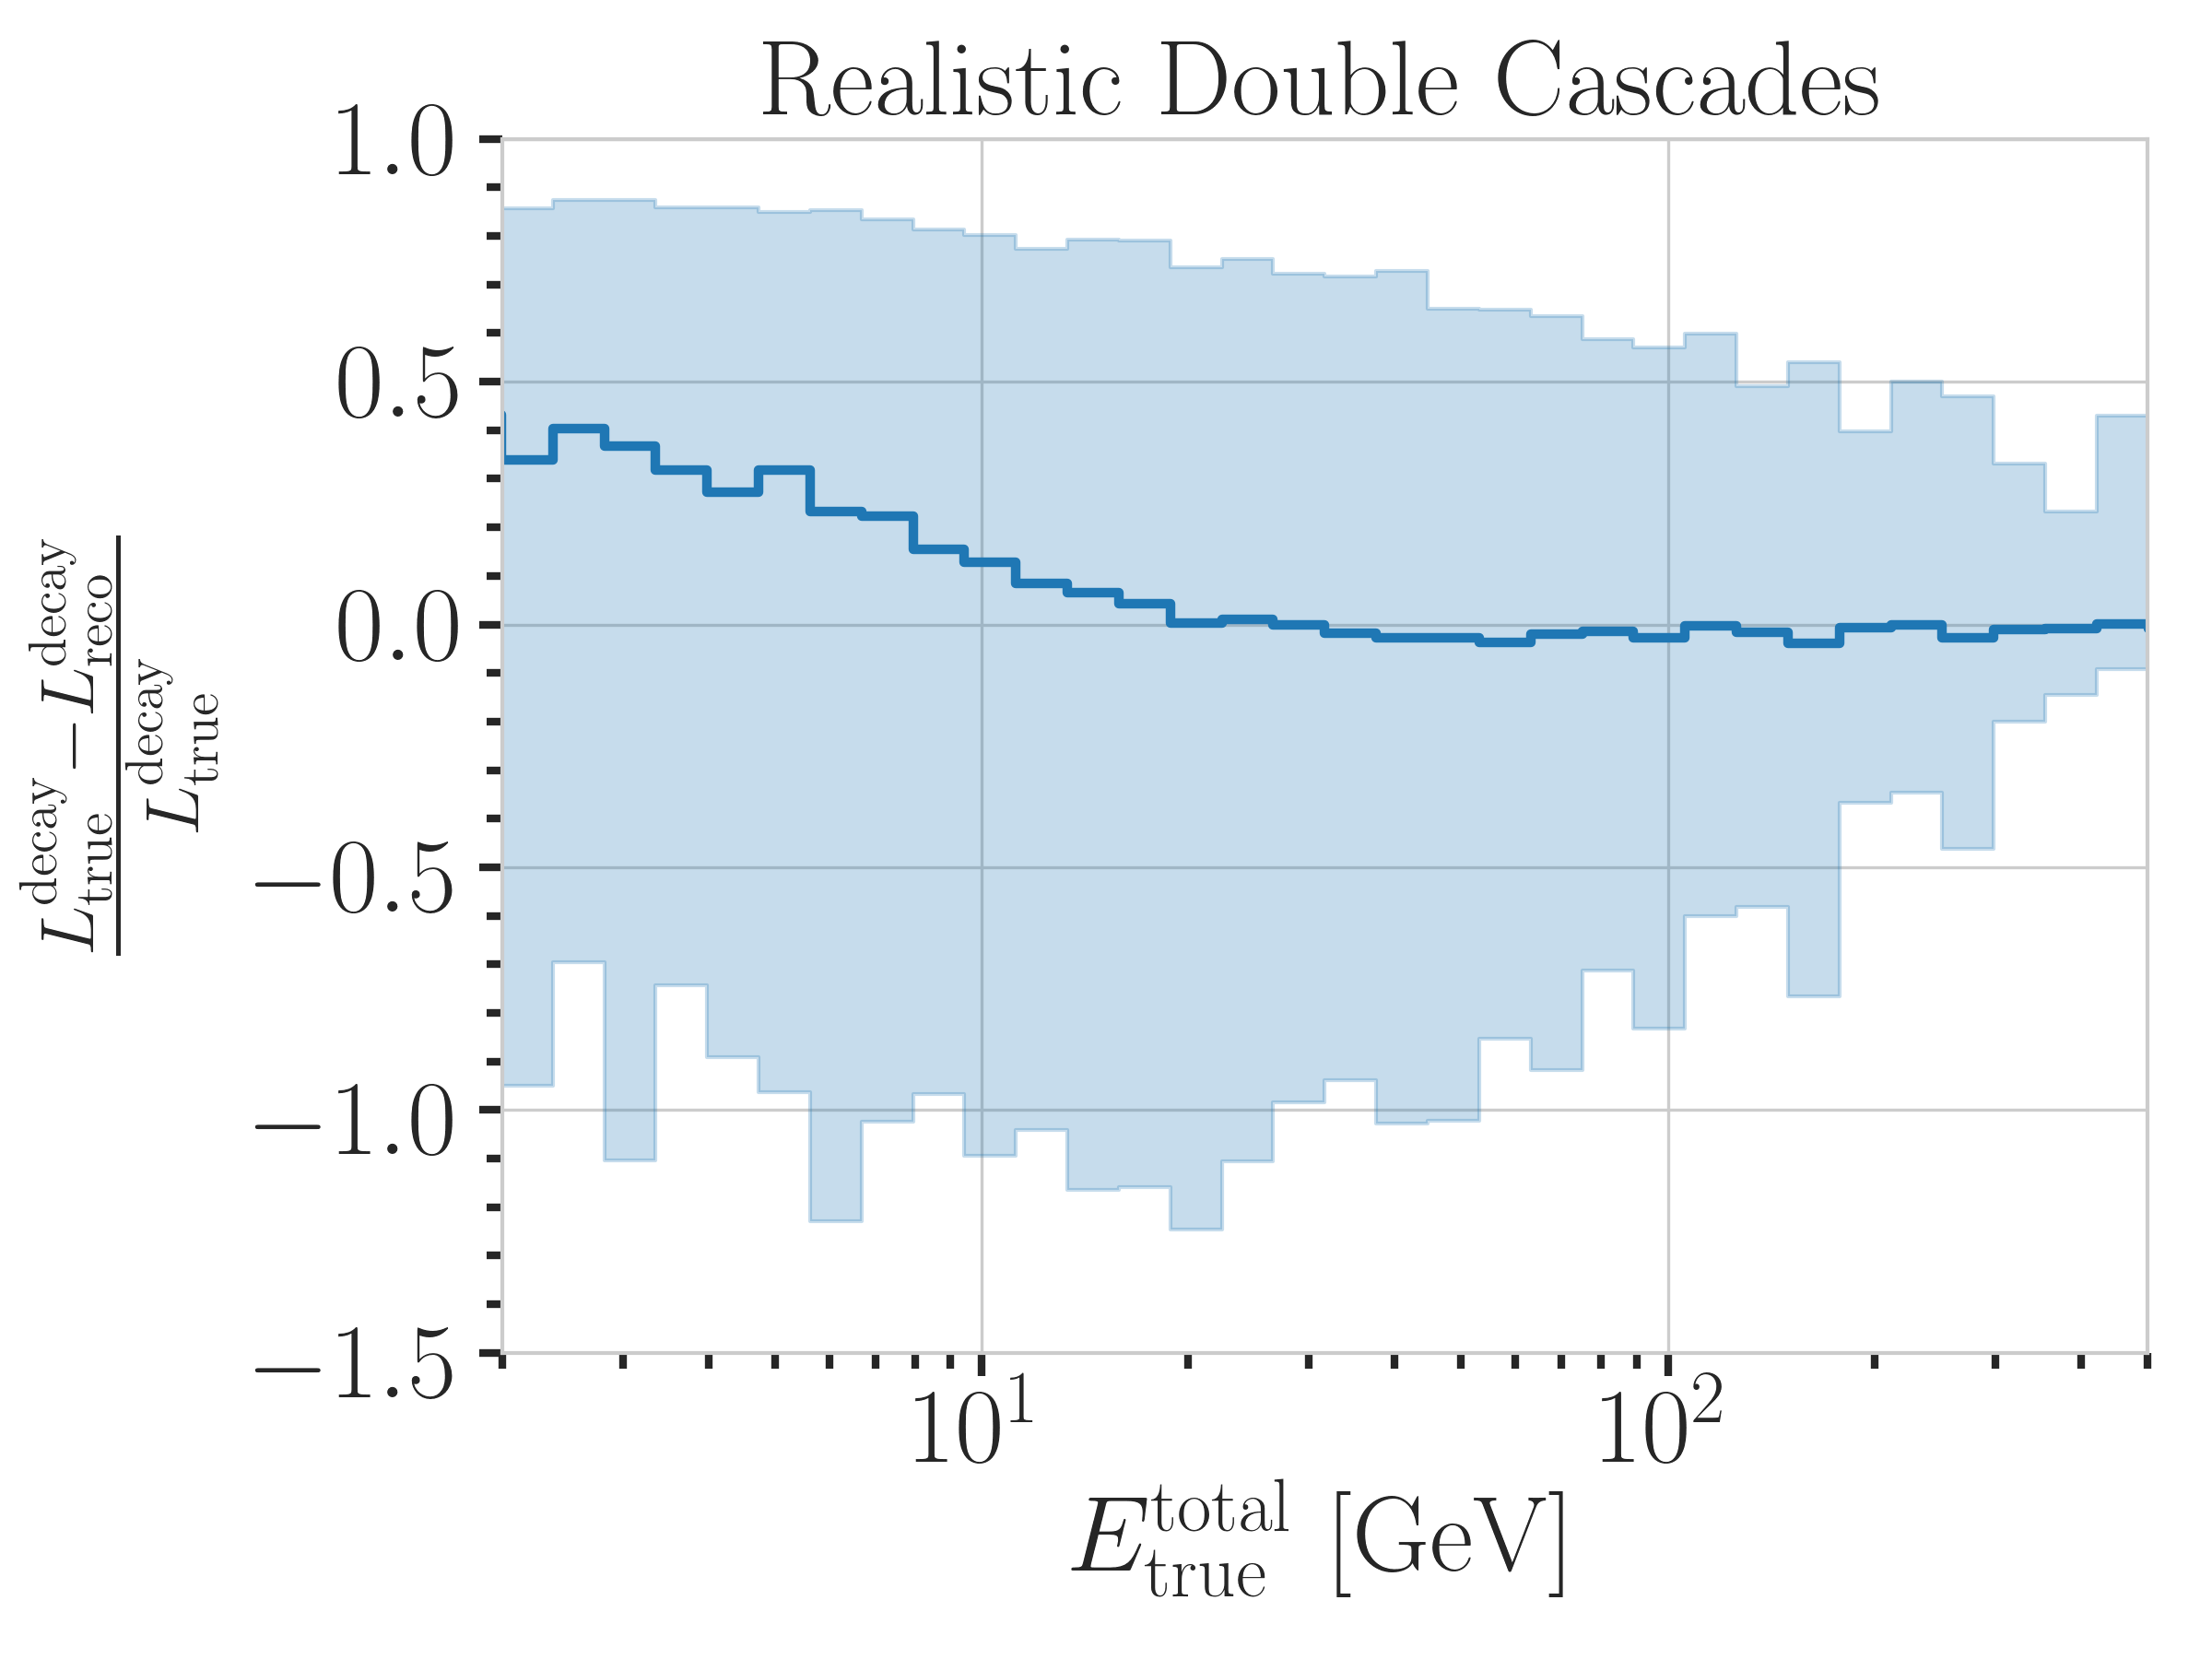
\includegraphics[width=0.49\linewidth]{figures/model_independent_simulation/results/realistic/resolutions/194603_median_decay_length_bias_vs_tot_energy_goodfit_log_unweighted.png}
    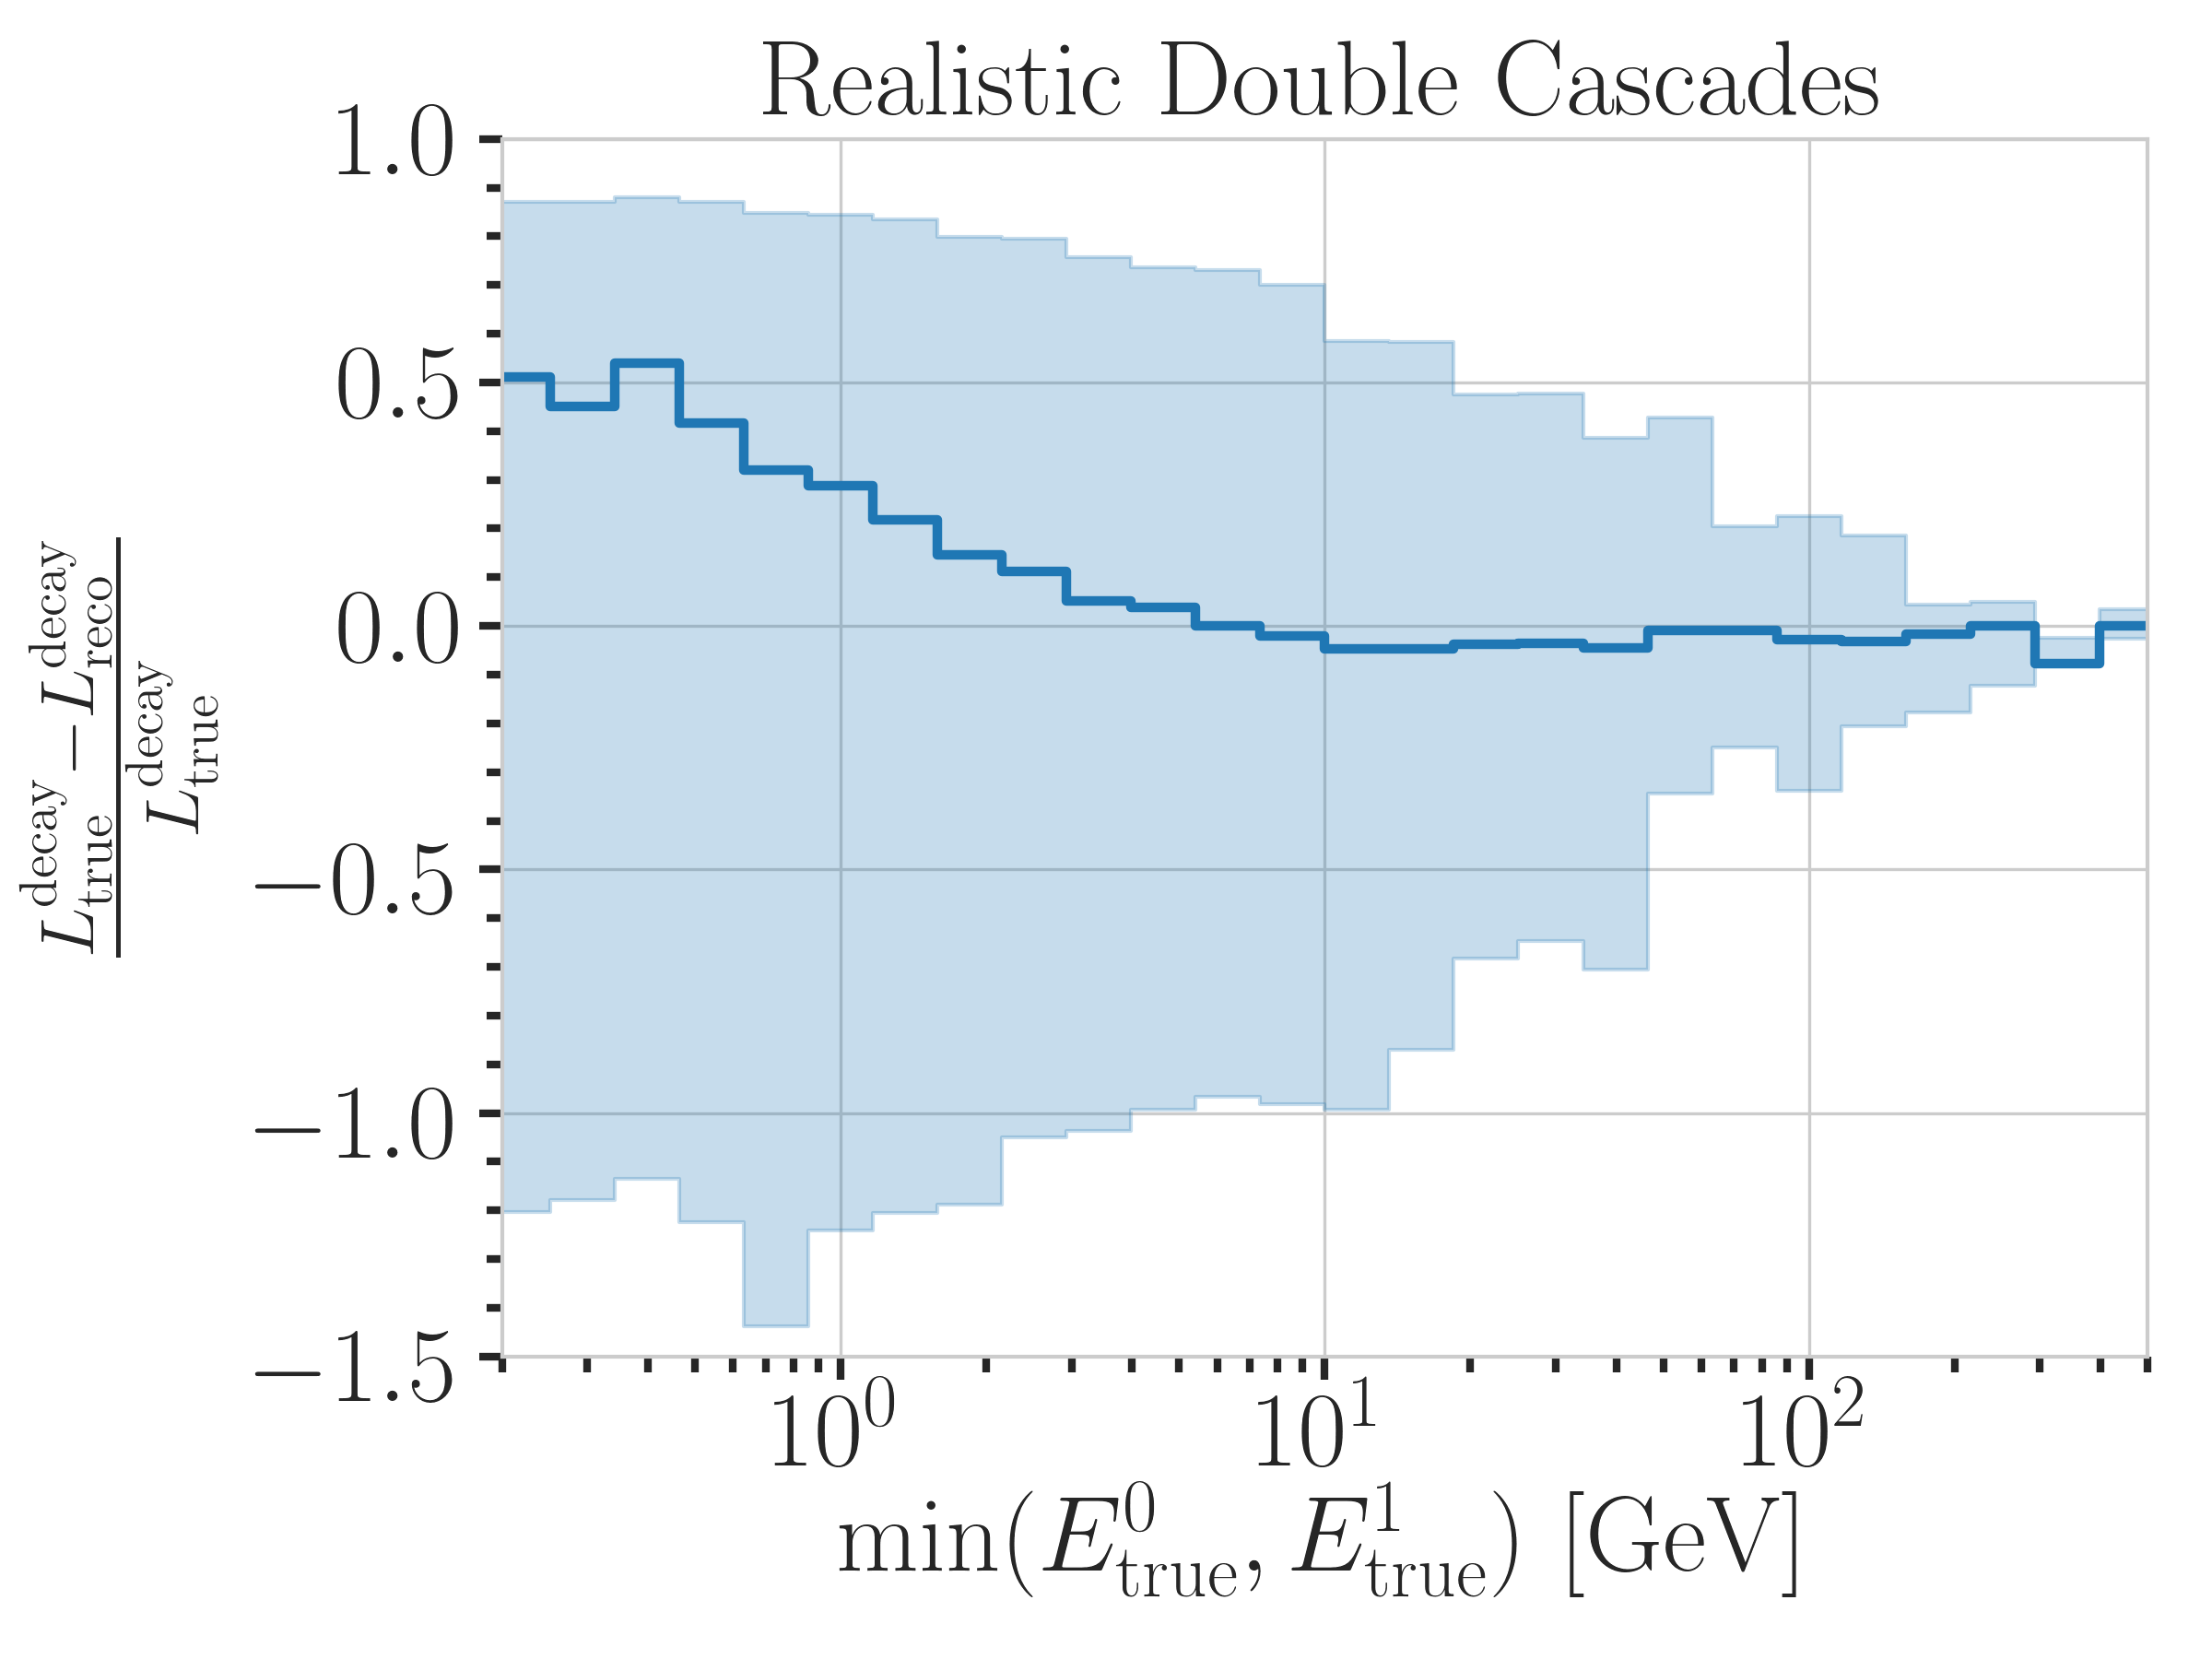
\includegraphics[width=0.49\linewidth]{figures/model_independent_simulation/results/realistic/resolutions/194603_median_decay_length_bias_vs_min_energy_goodfit_log_unweighted.png} 
    \caption[]{}
    \labfig{decay_length_bias_vs_energies}
\end{figure*}


\section{Low Energy Event Selection Efficiency}

\todo{Make plot to show efficiency of the OscNext selection for HNL events.}

\paragraph{Discussion ideas:}
\begin{itemize}
    \item At which level does the selection reduce the HNL the most?
    \item Is there a place to improve the HNL selection? (Might have to factor in the BG efficiency, as well..)
    \item What of this might change with Upgrade? (maybe rather for the discussion)
\end{itemize}

